% =====================================================================
% Master Thesis
% Automatic Training Set Expansion for Entity Matching
% Using LLM-Based Labeling and Web Retrieval
% Abdullah Momin (1869371), University of Mannheim
% =====================================================================
% Do not change document class, margins, fonts, etc.
\documentclass[a4paper,oneside,bibliography=totoc]{scrbook}

% some useful packages (add more as needed)
\usepackage[utf8]{inputenc}
\usepackage{graphicx}
\usepackage{latexsym}
\usepackage{amsmath}
\usepackage{amssymb}
\usepackage{tabularx}
\usepackage{booktabs}
\usepackage{multirow}
\usepackage{algorithm}
\counterwithin{algorithm}{chapter}
\usepackage{algorithmic}
\usepackage{csquotes}
\renewcommand{\algorithmiccomment}[1]{\hfill\textit{// #1}}
\usepackage[usenames,dvipsnames]{xcolor}
\usepackage[colorlinks,citecolor=Green]{hyperref}

% chicago citation style
\usepackage{natbib}
\bibliographystyle{chicagoa}
\setcitestyle{authoryear,round,semicolon,aysep={},yysep={,}} \let\cite\citep

% environments
\newtheorem{definition}{Definition}

% small helper for still-open sections
\newcommand{\pending}[1]{\begin{center}\fbox{\parbox{0.9\textwidth}{\textit{[This section will be completed once the corresponding experiment has finished. #1]}}}\end{center}}

\begin{document}

\frontmatter \subject{Master Thesis}
\title{Automatic Training Set Expansion for Entity Matching Using LLM-Based Labeling and Web Retrieval}
\author{Abdullah Momin\\
  (matriculation number 1869371)} \date{July 31, 2026}
\publishers{{\small Submitted to}\\
  Data and Web Science Group\\
  Prof.\ Dr.\ Christian Bizer\\
  University of Mannheim\\}
\maketitle

\chapter{Abstract}

Entity matching decides whether two records describe the same real-world object, for example whether two product offers from different shops refer to the same product. Transformer-based matchers such as Ditto reach strong results but need labeled training pairs, which are expensive to obtain. This thesis asks whether an existing training set can be expanded automatically, without further human labeling, and whether the expansion improves a RoBERTa-based matcher. We compare three expansion strategies on two benchmarks (WDC Products and DBLP-Scholar): (i) string-based augmentation that rewrites existing pairs with token-level edit operations, (ii) LLM-based augmentation that selects new candidate pairs via embedding blocking and active learning and labels them with a large language model acting as a teacher, and (iii) web retrieval augmentation that gathers new product offers and paper records from the web and again lets the LLM teacher label the resulting pairs.

The outcome is largely negative, and the reasons are instructive. Over three random seeds, no strategy beats the baseline on WDC Products (best mean gain +0.016 F1, not significant), and on DBLP-Scholar only string augmentation changes the result at all --- it makes it slightly worse (-0.008 F1). Even training on the union of all three additions, which overlap in zero pairs, only reproduces the best single strategy (+0.017 on WDC Products, statistically indistinguishable from string augmentation alone). Our analysis shows why: once the expansion is forced to be entity-disjoint from the test set, the candidate pool for LLM labeling contains almost no new positive pairs (5.6\% on WDC Products, 0\% on DBLP-Scholar), because on a closed benchmark nearly all true matches are already part of the labeled data. The teacher itself is not the problem: its labels agree with the ground truth in 97.1\% of cases (F1 0.862). Web retrieval does inject genuinely new positives, but the retrieved text comes from a different distribution than the benchmark records, and a follow-up experiment that rebalanced the web data and added LLM-generated hard negatives made results significantly worse rather than better. We situate these findings in a detailed comparison with DistillER \cite{zeakis2026distiller} and with \citet{steiner2026labeling}, whose label-replacement setting recovers over 99\% of the benchmark positives and therefore does not face the scarcity problem: expanding a training set is structurally harder than relabeling one. Along the way, the thesis documents an entity-leakage pitfall in augmentation pipelines, quantifies how single-seed evaluations produced conclusions that did not survive seed averaging, and argues for paired significance tests on shared test sets.

% table of contents
\begingroup%
\hypersetup{hidelinks}%
\tableofcontents%
\endgroup

\listoftables
\listoffigures

\mainmatter

% =====================================================================
\chapter{Introduction}
\label{ch:intro}
% =====================================================================

\section{Motivation}
\label{sec:motivation}

A large part of the value of data comes from combining it. Price comparison portals combine product offers from thousands of shops, bibliographic services combine publication records from different digital libraries, and companies merge customer databases after acquisitions. In all of these settings the same question appears again and again: do these two records describe the same real-world thing? This question is called entity matching (also record linkage or entity resolution), and it has been studied for over sixty years \cite{newcombe1959automatic,fellegi1969theory,christen2012data}.

The current state of the art treats entity matching as a binary classification problem over record pairs and solves it with pre-trained transformer language models. Ditto \cite{li2020deep}, which fine-tunes models such as RoBERTa \cite{liu2019roberta} on serialized record pairs, remains a strong and widely used reference point. The catch is the training data. Fine-tuning needs thousands of labeled pairs, and labeling pairs is slow, boring, and expensive work that requires some domain knowledge --- deciding whether two laptop offers describe the same configuration means reading model numbers, memory sizes, and bundle contents carefully. The cost of building training sets, not the model architecture, is today the main obstacle to using neural entity matching in practice \cite{barlaug2021neural}.

Two recent developments promise a way out. First, large language models (LLMs) have become good at entity matching themselves when prompted directly \cite{narayan2022can,peeters2023using,peeters2025entity}, which raises the possibility of using an LLM as a cheap annotator: let the LLM label pairs, and train a small, fast model on those labels. This is knowledge distillation in the classic sense of \citet{hinton2015distilling}, with the LLM as the teacher and the small model as the student. Two works pursue this direction and form the main points of comparison for this thesis: DistillER \cite{zeakis2026distiller} distills LLM labels into small student models across eight benchmarks, and \citet{steiner2026labeling} replace the human labels of existing benchmarks with LLM labels and measure how much downstream quality is lost. Second, the web itself is a source of additional records: for a product in the training set, other shops sell the same product and describe it differently, and a web search API can retrieve those descriptions.

This thesis combines both ideas and asks a question that sounds similar to prior work but differs in one important way. DistillER and \citet{steiner2026labeling} study \emph{replacement}: they take the pairs of an existing benchmark and relabel them with an LLM teacher. We study \emph{expansion}: we keep the existing human-labeled training set and try to add \emph{new} pairs on top of it --- pairs the benchmark does not contain, found either by blocking over the entity tables or by retrieving new records from the web, and labeled by the LLM teacher. Expansion is the scenario a practitioner actually faces: they already have some labeled data and want to know whether automatic methods can enlarge it profitably. As we will see, this seemingly small difference in framing has large consequences.

\section{Problem Statement and Research Questions}
\label{sec:problem}

We are given a training set $T = \{(l_i, r_i, y_i)\}$ of record pairs with binary labels ($y=1$: match, $y=0$: non-match), a validation set, and a held-out test set from the same benchmark. The task is to construct an expanded training set $T' \supseteq T$ automatically --- without any additional human labels --- such that a student model fine-tuned on $T'$ achieves higher F1 on the test set than the same model fine-tuned on $T$. The expansion must respect a hygiene constraint: it may not use any entity that only appears in the validation or test split, since otherwise the student would see held-out entity descriptions during training.

The thesis answers the following research questions:

\begin{itemize}
\item \textbf{RQ1:} Does simple string-based augmentation, which creates modified copies of existing pairs, improve the downstream F1 of a RoBERTa student?
\item \textbf{RQ2:} Does LLM-based augmentation, which selects new pairs from a blocked candidate pool via active learning and labels them with an LLM teacher, improve downstream F1?
\item \textbf{RQ3:} Does web retrieval augmentation, which obtains genuinely new records from outside the benchmark and pairs them with training entities, improve downstream F1?
\item \textbf{RQ4:} How do the expanded training sets compare in terms of label ratio, corner-case proportion, attribute coverage, and mutual overlap --- and how close do they come to the design targets set for them?
\item \textbf{RQ5:} How do the results relate to the label-replacement settings of DistillER \cite{zeakis2026distiller} and \citet{steiner2026labeling}, and what explains the differences?
\end{itemize}

\section{Contributions}
\label{sec:contributions}

The main contributions of this thesis are the following:

\begin{enumerate}
\item \textbf{A controlled comparison of three automatic expansion strategies} --- string-based, LLM-based with active learning, and web-retrieval-based --- on two benchmarks with different characteristics (WDC Products, an e-commerce benchmark with abundant hard cases, and DBLP-Scholar, a bibliographic benchmark near the performance ceiling). All strategies are evaluated with the same student model, the same three-layer evaluation scheme, three random seeds, and paired significance tests.
\item \textbf{A negative result with an explanation.} No expansion strategy robustly improves the student. We trace this to three separate mechanisms: positive scarcity in entity-disjoint candidate pools (the benchmark already contains nearly all true matches among its entities), a text-distribution mismatch between web-retrieved records and benchmark records, and a performance ceiling on DBLP-Scholar that leaves no room for improvement. We consider the first mechanism the central finding of the thesis: \emph{expanding} a closed benchmark honestly is structurally harder than \emph{relabeling} it, because the discoverable new pairs are almost all negatives.
\item \textbf{A quantified teacher-quality analysis.} Using the cluster ground truth of WDC Products, we measure the LLM teacher's labeling quality exactly (accuracy 0.971, F1 0.862, 2.9\% label noise) and show that teacher noise is not the bottleneck of LLM-based expansion.
\item \textbf{A methodological case study.} The first version of our LLM and web pipelines leaked held-out entities into the training data; we document the leak, the fix, and its effects. Similarly, several single-seed conclusions (including one apparently significant improvement) did not survive averaging over three seeds. Both episodes are reported openly because they are easy mistakes to make and their effects were large enough to flip conclusions.
\item \textbf{An in-depth comparison with two related systems}, DistillER and \citet{steiner2026labeling}, that reconciles apparently contradictory numbers by making training budgets and test-set versions explicit, and positions augmentation and replacement as two distinct regimes of LLM-teacher entity matching.
\end{enumerate}

\section{Outline}
\label{sec:outline}

Chapter~\ref{ch:related_work} introduces the entity matching problem and reviews related work on neural matchers, data augmentation, LLMs for data integration, knowledge distillation, and active learning. Chapter~\ref{ch:datasets} describes the two benchmarks, their preprocessing, and a split-hygiene analysis whose results matter later. Chapter~\ref{ch:methods} presents the student model and the three expansion pipelines in detail, including the entity-disjointness policy. Chapter~\ref{ch:setup} defines the experimental setup: training configuration, metrics, the multi-seed protocol, significance testing, and the three-layer evaluation scheme. Chapter~\ref{ch:results} reports the main results. Chapter~\ref{ch:iteration} covers the second experimental iteration requested by the supervisor: hard-negative mining for DBLP-Scholar, a rebalanced web augmentation variant with generated hard negatives, training on the union of all augmentation sets, and a low-resource ablation that is still running at the time of writing. Chapter~\ref{ch:comparison} compares our findings with DistillER and \citet{steiner2026labeling}. Chapter~\ref{ch:discussion} discusses the mechanisms behind the results and the limitations of the study, and Chapter~\ref{ch:conclusions} concludes.

% =====================================================================
\chapter{Background and Related Work}
\label{ch:related_work}
% =====================================================================

This chapter first fixes terminology and describes the standard entity matching pipeline (Section~\ref{sec:preliminaries}). It then reviews the lines of work this thesis builds on: neural entity matching (Section~\ref{sec:rw_neural}), data augmentation (Section~\ref{sec:rw_augmentation}), large language models for entity matching (Section~\ref{sec:rw_llm}), knowledge distillation with LLM teachers (Section~\ref{sec:rw_distillation}), and active learning (Section~\ref{sec:rw_al}). Section~\ref{sec:rw_positioning} summarizes how the thesis relates to this landscape.

\section{Preliminaries}
\label{sec:preliminaries}

\begin{definition}[Entity Matching]
Given two collections of records $A$ and $B$, where each record describes a real-world entity through a set of attribute values, entity matching is the task of finding all pairs $(a, b) \in A \times B$ such that $a$ and $b$ refer to the same real-world entity.
\end{definition}

In practice the task is solved in two stages \cite{christen2012data,papadakis2020blocking}. The first stage, \emph{blocking}, cheaply discards the vast majority of the $|A| \times |B|$ possible pairs so that only plausible candidates remain; without blocking, even the moderately sized datasets used in this thesis would produce up to 168 million pairs. The second stage, \emph{matching}, applies a more expensive classifier to each surviving candidate pair and outputs a binary decision. This thesis is concerned with the matching stage: all benchmarks used here provide fixed sets of candidate pairs with human labels, and the matcher is trained and evaluated on those pairs. Blocking still appears in one place, though --- our LLM-based expansion pipeline uses embedding-based blocking to generate its own candidate pairs (Section~\ref{sec:method_llm}).

Matching quality is measured on the positive (match) class. With $tp$, $fp$, and $fn$ denoting true positives, false positives, and false negatives, precision is $P = tp/(tp+fp)$, recall is $R = tp/(tp+fn)$, and the F1 score is their harmonic mean, $F_1 = 2PR/(P+R)$. F1 on the match class is the standard headline metric in entity matching because the class distribution is heavily skewed toward non-matches \cite{kopcke2010evaluation}, and we follow that convention throughout.

Two properties of a benchmark deserve attention because they will play a large role later. First, a benchmark is \emph{entity-disjoint} if no entity that appears in the training split also appears in the validation or test split. Entity-disjoint test sets measure generalization to unseen entities; non-disjoint test sets partly measure memorization. Second, benchmarks differ in their share of \emph{corner cases}: pairs that are hard because surface similarity and true label disagree --- highly similar non-matches (for example, the 500\,GB and 1\,TB variants of the same SSD) and dissimilar matches (the same product described with completely different words).

\section{From Rule-Based Systems to Neural Entity Matching}
\label{sec:rw_neural}

Entity matching predates machine learning. \citet{newcombe1959automatic} already linked vital records automatically in 1959, and \citet{fellegi1969theory} gave the problem its classic probabilistic formulation, modeling the odds that agreement patterns between record fields arise from a true match versus a coincidence. Decades of subsequent work refined similarity functions, blocking schemes, and rule-based decision models; \citet{elmagarmid2007duplicate} and \citet{christen2012data} survey this period. Systems such as Magellan \cite{konda2016magellan} packaged the resulting best practices --- feature engineering over string similarity measures, followed by a conventional classifier such as a random forest --- into a usable toolchain, and this feature-based paradigm remains a strong baseline on structured data.

Deep learning entered the field with DeepER \cite{ebraheem2018distributed} and DeepMatcher \cite{mudgal2018deep}, which replaced hand-crafted similarity features with learned representations built from word embeddings and recurrent networks. DeepMatcher's design-space study showed that the gains of deep models over Magellan were largest on textual and dirty data --- exactly the settings where hand-crafted features struggle --- and small on clean, structured data. The next step followed the general trajectory of NLP: pre-trained transformers \cite{vaswani2017attention,devlin2019bert}. \citet{brunner2020entity} showed that fine-tuning BERT-family models on serialized record pairs beats previous architectures, and Ditto \cite{li2020deep} turned this into the reference architecture that this thesis also uses. Ditto serializes each record into a tagged string (\texttt{COL} \emph{attribute} \texttt{VAL} \emph{value} \ldots), concatenates the two records of a pair with a separator token, and fine-tunes a pre-trained language model such as RoBERTa \cite{liu2019roberta} with a binary classification head. Ditto also introduced three optimizations --- domain knowledge injection, summarization of long values, and data augmentation --- of which the last is a direct ancestor of our first expansion strategy. \citet{barlaug2021neural} give a survey of this generation of matchers.

The important background fact for this thesis is that transformer matchers are data-hungry. Ditto's reported advantage over DeepMatcher grows with training set size, and on small training sets fine-tuning is unstable: as we will see in Chapter~\ref{ch:results}, the same model trained on the same 2{,}500 pairs with different random seeds can vary by more than 0.02 F1. This data hunger motivates the entire premise of the thesis --- and the seed variance shapes its evaluation protocol.

\section{Benchmarks}
\label{sec:rw_benchmarks}

Most published entity matching results use the benchmark collection assembled around Magellan and DeepMatcher \cite{konda2016magellan,mudgal2018deep}, which includes the bibliographic DBLP-Scholar dataset used in this thesis, and the WDC product corpora \cite{primpeli2019wdc}. \citet{kopcke2010evaluation} established DBLP-Scholar as a standard task: matching computer science publication records from DBLP against records crawled from Google Scholar, where Scholar records are notoriously noisy (truncated author lists, garbled venues, missing years).

WDC Products \cite{peeters2024wdc} is a newer benchmark built from product offers on the web that carry schema.org annotations, which supply cluster identifiers as ground truth. Its distinguishing feature is that difficulty is a controlled dimension: the benchmark comes in variants with a chosen share of corner cases (we use the hardest, ``80\% corner cases'' variant), with seen or unseen test entities (we use unseen, i.e.\ the entity-disjoint variant), and with three training sizes (we use small). This controllability is why WDC Products is our primary benchmark: it was explicitly designed to punish matchers that rely on surface similarity, which is the failure mode that data augmentation is supposed to address.

\section{Data Augmentation for Entity Matching}
\label{sec:rw_augmentation}

Data augmentation enlarges a training set by transforming existing examples in label-preserving ways. In NLP, simple token-level operations --- synonym replacement, random insertion, swap, and deletion --- can help small-data text classification \cite{wei2019eda}; \citet{shorten2021text} survey the area. Ditto \cite{li2020deep} adapted this idea to entity matching with operators that respect the structure of serialized records: deleting spans of value tokens, shuffling token spans, dropping whole attributes, and swapping the two records of a pair. The intuition is that a matcher should not change its decision because a word was dropped or an attribute reordered, so training on such perturbed copies teaches invariance.

Rotom \cite{miao2021rotom} took augmentation a step further with a meta-learning framework that learns which augmentation policies to apply and how to weight the generated examples, reporting gains over fixed policies on entity matching among other tasks. Our string-based strategy (Section~\ref{sec:method_string}) deliberately stays with Ditto's fixed operators: it is the simple, cheap, LLM-free baseline against which the two more elaborate strategies must justify their cost.

A shared limitation of all perturbation-based augmentation is that it cannot create genuinely new information. A perturbed copy of a pair contains the same entities, the same decisive attributes, and the same label; the model sees more variation but no new facts. The two other strategies in this thesis are attempts to break this limitation --- by pairing entities in new combinations (LLM-based expansion) and by importing entirely new records from outside the benchmark (web retrieval).

\section{Large Language Models for Entity Matching}
\label{sec:rw_llm}

\citet{narayan2022can} first showed that large autoregressive language models can perform data integration tasks, including entity matching, from prompts with few or no examples. \citet{peeters2023using} evaluated ChatGPT on product matching and found it competitive with fine-tuned baselines that had seen thousands of labeled pairs; the extended study of \citet{peeters2025entity} systematically compared prompt designs, model families, and fine-tuning across benchmarks, and found that hosted frontier models match or exceed fine-tuned RoBERTa on many datasets, with the practical drawbacks of cost and latency per pair.

These results changed the economics of the field. If an LLM can label a pair for a fraction of a cent at near-human quality, human annotation stops being the only way to create training data. Two consequences are being explored in the literature. The first is to use the LLM directly as the matcher --- accurate but expensive at scale, since every candidate pair triggers an API call at inference time. The second is to use the LLM as an annotator that creates training data for a small student model, which is then cheap at inference time. This second route is the one this thesis takes, and it leads directly to knowledge distillation.

\section{Knowledge Distillation and LLM Teachers}
\label{sec:rw_distillation}

Knowledge distillation \cite{hinton2015distilling} originally described training a small student network to imitate the output distribution of a large teacher network; DistilBERT \cite{sanh2019distilbert} is a well-known application to pre-trained language models, and \citet{gou2021knowledge} survey the many variants. In the looser sense used in recent entity matching work --- and in this thesis --- distillation means training a student on \emph{labels produced by a teacher} rather than on ground-truth labels. The teacher is a prompted LLM, the student a fine-tuned compact model, and the interesting question is how much quality survives the noisy teacher.

Two works define the state of the art here, and Chapter~\ref{ch:comparison} compares against both in detail; we summarize them briefly. DistillER \cite{zeakis2026distiller} distills the labels of a Qwen-2.5 32B teacher into small students (RoBERTa among them) across eight standard benchmarks in a deliberately low-resource setting where only about 10\% of entities are available for training-pair construction. Their central result is encouraging for distillation: the RoBERTa student reaches an average F1 of 0.69 with teacher labels versus 0.66 with ground-truth labels over the eight datasets --- noisy LLM labels were on average no worse than human labels for the student, and on some product datasets they were better. They also study unsupervised selection of pairs to label, finding similarity-ranking-based selection that roughly maintains a 3:1 negative-to-positive ratio to be the most reliable.

\citet{steiner2026labeling} ask the replacement question directly: if we relabel the training pairs of existing benchmarks with an LLM teacher (GPT-based, among others), how much downstream F1 does a student like Ditto lose compared to training on the original human labels? Their answer is: little --- across benchmarks including WDC Products and DBLP-Scholar, students trained on machine labels come close to students trained on human labels. They also compare several strategies for \emph{choosing} which pairs to label, including an active-learning variant with an ensemble of feature-based classifiers; that variant is the direct blueprint for our LLM-based expansion pipeline (Section~\ref{sec:method_llm}). A crucial detail, easy to overlook and central to this thesis, is that their candidate pools are built from the benchmark's own pair universe and recover 99.56--99.92\% of the original positive pairs. Their teacher relabels pairs the benchmark already knew about. Whether an LLM teacher can find \emph{new} matches beyond the benchmark's own pairs is exactly the question their setup does not pose --- and ours does.

\section{Active Learning for Entity Matching}
\label{sec:rw_al}

Active learning selects the most informative examples to label next, instead of labeling at random \cite{settles2009active}. In entity matching it has a long history because labeling budgets are the binding constraint; \citet{meduri2020comprehensive} benchmark many combinations of learners and selection strategies, and \citet{kasai2019low} combine transfer learning with active learning for deep matchers under tight budgets. \citet{primpeli2021graph} exploit the graph structure of match decisions to improve selection. The selection principle used in this thesis is committee-based uncertainty \cite{settles2009active}: train several diverse classifiers on the labeled pool, and query the pairs on which the committee disagrees most. Following \citet{steiner2026labeling}, our committee consists of a random forest \cite{breiman2001random}, XGBoost \cite{chen2016xgboost}, gradient boosting \cite{friedman2001greedy}, and logistic regression, all over classic string-similarity features --- a deliberately cheap committee, since its only job is to point the expensive LLM teacher at informative pairs.

\section{Positioning of This Thesis}
\label{sec:rw_positioning}

Against this backdrop, the gap this thesis addresses can be stated precisely. Prior work has shown that LLM teachers can \emph{replace} human annotators on existing benchmark pairs at small quality loss \cite{steiner2026labeling,zeakis2026distiller}, and that perturbation-based augmentation can help transformer matchers \cite{li2020deep,miao2021rotom}. What has not been studied is the \emph{expansion} setting: keeping the human training set and adding new, automatically discovered, LLM-labeled pairs on top --- either from the benchmark's own entity tables via blocking, or from outside the benchmark via web retrieval. Expansion differs from replacement in what the candidate pool can contain, and it differs from perturbation in that it can, in principle, add new information. The thesis evaluates both new routes against the perturbation baseline under identical conditions, imposes the entity-disjointness hygiene that the setting requires, and explains the results through the composition of the candidate pools rather than only through downstream F1.


% =====================================================================
\chapter{Datasets}
\label{ch:datasets}
% =====================================================================

We evaluate on two benchmarks that were chosen to be as different as possible in the properties that matter for augmentation: WDC Products, an e-commerce benchmark deliberately built around hard cases with plenty of headroom for improvement, and DBLP-Scholar, a bibliographic benchmark on which transformer matchers already operate near their ceiling. This chapter describes both datasets, the shared serialization format, and a split-hygiene analysis that turned out to be important for interpreting the results.

\section{WDC Products}
\label{sec:data_wdc}

WDC Products \cite{peeters2024wdc} contains product offers extracted from web pages with schema.org annotations. Offers that carry the same product identifier (e.g.\ a GTIN or MPN) form clusters, and these cluster memberships serve as ground truth: two offers match if and only if they belong to the same cluster. Each offer has the attributes \texttt{brand}, \texttt{title}, \texttt{description}, \texttt{price}, and \texttt{priceCurrency}. The benchmark spans many product categories, with a concentration of electronics and computer hardware --- a domain where near-identical product variants (storage sizes, colors, bundled accessories) make matching genuinely difficult.

We use the configuration that is hardest and cleanest at the same time: the \textbf{80\% corner-case} variant (80\% of the pairs are hard positives or hard negatives by the benchmark's own construction), the \textbf{unseen} test set (test entities are disjoint from training entities), and the \textbf{small} training size. Table~\ref{tab:datasets} shows the split statistics. Two numbers deserve emphasis. First, the training set is small: 2{,}500 pairs over roughly 1{,}000 distinct entities --- this is the low-resource setting in which augmentation should matter most. Second, the positive rate differs between splits: 20.0\% of training and validation pairs are matches, but only 11.1\% of test pairs are. This \emph{prior shift} is a property of the published benchmark, not of our processing, and Section~\ref{sec:results_threshold} shows that it acts as a hidden ceiling on test F1.

\begin{table}[tb]
  \centering
  \begin{tabular}{llrrrr}
    \toprule
    \textbf{Dataset} & \textbf{Split} & \textbf{Pairs} & \textbf{Matches} & \textbf{Non-matches} & \textbf{\% Positive} \\
    \midrule
    WDC Products & train & 2{,}500 & 500 & 2{,}000 & 20.0 \\
                 & valid & 500 & 100 & 400 & 20.0 \\
                 & test  & 4{,}500 & 500 & 4{,}000 & 11.1 \\
    \midrule
    DBLP-Scholar & train & 17{,}223 & 3{,}207 & 14{,}016 & 18.6 \\
                 & valid & 5{,}742 & 1{,}070 & 4{,}672 & 18.6 \\
                 & test  & 5{,}742 & 1{,}070 & 4{,}672 & 18.6 \\
    \bottomrule
  \end{tabular}
  \caption{Split statistics of the two benchmarks as used in this thesis. WDC Products is the 80\%-corner-case, small-training, unseen-test configuration.}
  \label{tab:datasets}
\end{table}

\section{DBLP-Scholar}
\label{sec:data_dblp}

DBLP-Scholar \cite{kopcke2010evaluation} matches publication records from the DBLP bibliography (2{,}616 records in the version used here) against records crawled from Google Scholar (64{,}263 records). Each record has the attributes \texttt{title}, \texttt{authors}, \texttt{venue}, and \texttt{year}. The Scholar side is noisy in characteristic ways: author lists are abbreviated or truncated, venue strings are inconsistent, years are missing. We use the standard split from the Magellan/DeepMatcher benchmark collection \cite{mudgal2018deep}, with 17{,}223 training, 5{,}742 validation, and 5{,}742 test pairs (Table~\ref{tab:datasets}).

DBLP-Scholar plays the role of a contrast dataset in this thesis. Fine-tuned transformers reach F1 around 0.95 on it, so there is little headroom; its pairs are mostly either clearly matching or clearly different (few corner cases, as quantified in Section~\ref{sec:results_layer2}); and its split has hygiene issues that the next section makes precise. If augmentation helps anywhere, it should be on WDC Products; DBLP-Scholar tests whether augmentation at least does no harm near the ceiling.

\section{Serialization Format}
\label{sec:data_serialization}

Both datasets are converted into Ditto's serialization format \cite{li2020deep}. Each record becomes a string of the form

\begin{center}
\texttt{COL title VAL Querying and Mining Data Streams ... COL venue VAL SIGMOD COL year VAL 2002}
\end{center}

and a pair is stored as the two serialized records plus a tab-separated binary label. WDC Products records serialize the attributes \texttt{brand}, \texttt{title}, \texttt{description}, \texttt{price}, and \texttt{priceCurrency}; DBLP-Scholar records serialize \texttt{title}, \texttt{authors}, \texttt{venue}, and \texttt{year}. Missing values become empty strings after the \texttt{VAL} marker. All training files produced in this thesis --- the original splits and every augmented variant --- use exactly this format, so any of them can be fed to the same training script unchanged.

\section{Split Hygiene Analysis}
\label{sec:data_hygiene}

Because the whole point of this thesis is to add training pairs, we need to know precisely what the existing splits do and do not share. We verified three properties directly on the raw data; the results are summarized in Table~\ref{tab:hygiene} and referenced repeatedly in later chapters.

\begin{table}[tb]
  \centering
  \begin{tabular}{lrr}
    \toprule
    & \textbf{WDC Products} & \textbf{DBLP-Scholar} \\
    \midrule
    Test entities also in train (left)  & 0 (0.0\%) & 1{,}588 / 1{,}708 (93.0\%) \\
    Test entities also in train (right) & 0 (0.0\%) & 2{,}502 / 3{,}938 (63.5\%) \\
    Shared train--test pairs (by record ID) & 0 & 0 \\
    Shared train--test pairs (by exact text) & 0 & 186 (3.2\% of test) \\
    Positive rate train / test & 20.0\% / 11.1\% & 18.6\% / 18.6\% \\
    \bottomrule
  \end{tabular}
  \caption{Split hygiene of the two benchmarks, computed from the raw data. WDC Products is fully entity-disjoint; DBLP-Scholar is not, and additionally contains 186 test pairs whose serialized text is identical to a training pair.}
  \label{tab:hygiene}
\end{table}

\textbf{WDC Products is clean.} No entity from the test or validation split appears in training, no pair is shared between splits by ID, and no pair is shared by text either. Test performance on WDC Products therefore measures generalization to genuinely unseen products.

\textbf{DBLP-Scholar is not entity-disjoint.} 93.0\% of the DBLP-side test entities and 63.5\% of the Scholar-side test entities also appear somewhere in the training split. This is a known property of the pair-level random splits in the Magellan benchmark collection, not an error in our processing, but it matters for interpretation: a model can succeed on much of the DBLP-Scholar test set by recognizing entities it has already seen, so the near-ceiling baseline F1 of about 0.956 partly reflects memorization.

\textbf{DBLP-Scholar contains text-identical cross-split pairs.} While no pair is shared between train and test at the level of record IDs, the entity tables contain duplicate records --- the same paper appearing under different IDs. As a result, 186 test pairs (3.2\% of the test set) are \emph{textually identical} to a training pair, along with 160 train--validation and 64 test--validation duplicates. We state this precisely as ``0 ID-level shared pairs; 186 text-identical pairs'', because the ID-level statement alone would give a false impression of cleanliness: for a text-based matcher, a textually identical pair is the same input regardless of its ID.

These facts shape the thesis in two ways. First, they define the hygiene bar for our own pipelines: on WDC Products, augmentation must use training entities only, preserving full disjointness; on DBLP-Scholar, where the baseline itself is not disjoint, augmentation must at least not use any entity that appears \emph{exclusively} in validation or test (Section~\ref{sec:method_disjoint}). Second, they pre-register an interpretation caveat: improvements are hard to obtain on DBLP-Scholar not only because the task is easy for transformers, but because part of the test set is effectively already known to the model.

% =====================================================================
\chapter{Methods: Three Strategies for Training Set Expansion}
\label{ch:methods}
% =====================================================================

This chapter describes the student model and the three expansion pipelines. Throughout, we use the distillation terminology introduced in Section~\ref{sec:rw_distillation}: the large language model that labels pairs is the \emph{teacher}, and the RoBERTa matcher trained on the resulting data is the \emph{student}. Section~\ref{sec:method_requirements} states the design requirements the expanded training sets should meet. Section~\ref{sec:method_student} defines the student. Sections~\ref{sec:method_string} to~\ref{sec:method_web} present the three pipelines, and Section~\ref{sec:method_disjoint} describes the entity-disjointness policy that all pipelines must obey --- including the leakage incident that motivated its strict enforcement.

\section{Design Requirements for the Expanded Training Sets}
\label{sec:method_requirements}

An expanded training set should not just be bigger; it should be bigger in the right way. Based on the properties that make entity matching training sets effective --- and on explicit requirements formulated by the thesis supervisor --- the pipelines were designed toward the following targets:

\begin{itemize}
\item \textbf{Label ratio:} roughly 1:3 positive to negative pairs (25\% match rate), close to the ratio of the original training sets and consistent with what DistillER found to work for ranking-based selection \cite{zeakis2026distiller}.
\item \textbf{Corner cases:} 40--50\% of the added pairs should be hard --- positives with low surface similarity or negatives with high surface similarity --- since these are the pairs that teach a matcher something beyond token overlap.
\item \textbf{Diversity:} no single entity cluster, brand, or category should dominate the added pairs.
\item \textbf{Decisive attribute coverage} (WDC Products): the added pairs should cover variation in color, memory/storage, size, bundle contents, edition, and model number --- the attributes that decide hard product cases.
\item \textbf{Low label noise:} the teacher's prompt must be designed carefully, and teacher labels must be checked against ground truth where possible (Section~\ref{sec:setup_teacher}).
\item \textbf{Entity-disjointness:} the added pairs may only use entities from the training split (Section~\ref{sec:method_disjoint}).
\end{itemize}

Whether these targets were met is itself an empirical question, answered by the second evaluation layer in Section~\ref{sec:results_layer2}. Anticipating one result: the corner-case target turned out to be structurally out of reach once entity-disjointness is enforced, and understanding why is one of the main findings of the thesis.

\section{The Student Model}
\label{sec:method_student}

The student is a \texttt{roberta-base} model \cite{liu2019roberta} with a two-class classification head, fine-tuned on serialized record pairs --- the Ditto architecture \cite{li2020deep} reimplemented with current Hugging Face APIs \cite{wolf2020transformers}. A pair is encoded as \texttt{[CLS] left [SEP] right [SEP]}, truncated to 256 tokens, and classified as match or non-match. The original Ditto codebase targets Python~3.7 and outdated library versions; we use it as an architectural reference only and train with the standard \texttt{Trainer} (AdamW \cite{loshchilov2019decoupled}, weight decay 0.01, warmup of 100 steps). Full hyperparameters are listed in Chapter~\ref{ch:setup} and Appendix~\ref{app:hyperparams}.

One adaptation matters for WDC Products. With a 20\% positive rate and a small training set, the default cross-entropy objective produced a student biased against the minority match class. We therefore train a class-weighted variant for WDC Products, weighting each class inversely proportional to its frequency ($w_c = n/(2 n_c)$). This raised baseline F1 from 0.608 to 0.641 in the initial single-seed configuration and is used consistently for all WDC Products runs (marked with the suffix \texttt{\_cw} in result tables). DBLP-Scholar, with more data and a milder imbalance, did not benefit from class weighting, so its runs use the plain objective.

The student, its hyperparameters, its validation-based model selection, and its evaluation are held \emph{fixed} across all experiments. The only thing that varies between runs is the training file. This is the design principle of the whole thesis: every comparison is a comparison between training sets, not between models.

\section{Strategy 1: String-Based Augmentation}
\label{sec:method_string}

The first strategy is the classic one, ported from Ditto's augmentation module \cite{li2020deep}. It operates directly on the serialized strings and creates modified copies of existing training pairs. Three operators are used, each of which only ever touches value tokens --- the \texttt{COL}/\texttt{VAL} structure markers and attribute names are never modified, so every augmented string remains a valid serialization:

\begin{itemize}
\item \textbf{Span deletion (\texttt{del}):} delete a random span of 1--2 consecutive value tokens.
\item \textbf{Span shuffle (\texttt{swap}):} shuffle a random span of 2--4 consecutive value tokens in place.
\item \textbf{Attribute drop (\texttt{drop\_col}):} remove one attribute block entirely, preferring short attributes (at most 8 tokens) so that little information is lost.
\end{itemize}

Following Ditto's RandAugment-style \texttt{all} mode, each augmented record receives three operations drawn at random from this set. For every training pair, one augmented copy is created by independently augmenting the left and the right record while keeping the label. The output file contains the original pairs followed by the augmented copies, doubling the training set: 5{,}000 pairs for WDC Products and 34{,}446 for DBLP-Scholar.

The underlying assumption is label preservation: dropping a couple of tokens or reordering a span should not turn a match into a non-match. This is usually true, but not always --- deleting exactly the token \texttt{500GB} from one side of a hard negative can remove the only evidence of the non-match. We accept this small noise rate, as Ditto does, and note that the risk is highest precisely on corner cases. String augmentation adds no new entities, no new pairings, and no new labels; it is the control condition that any more expensive strategy must beat.

\section{Strategy 2: LLM-Based Augmentation with Active Learning}
\label{sec:method_llm}

The second strategy creates genuinely \emph{new} pairs --- pairings of training entities that the benchmark does not contain --- and labels them with the LLM teacher. The pipeline follows the active-learning recipe of \citet{steiner2026labeling} in four steps: embedding-based blocking builds a candidate pool, a seeding step labels an initial set of pairs, an active-learning loop iteratively labels the most uncertain candidates, and the labeled pairs are appended to the original training set. The teacher for all labeling steps is Claude (\texttt{claude-sonnet-4-6}), prompted per pair with the templates shown in Appendix~\ref{app:prompts}.

\subsection{Step 1: Embedding-Based Blocking}
\label{sec:method_llm_blocking}

All entity records are embedded with the sentence-transformer \texttt{all-MiniLM-L6-v2} \cite{reimers2019sentence,wang2020minilm}, applied to the same serialized text the student sees. For each left entity, the $k=20$ nearest right-side neighbors by cosine similarity form the raw candidate set. This produced 57{,}920 raw candidate pairs for WDC Products and 52{,}320 for DBLP-Scholar.

\subsection{Step 2: Filtering the Pool}
\label{sec:method_llm_filter}

Two filters are applied to the raw candidates. First, every pair that already appears in the benchmark --- in train, validation, or test --- is removed, because the goal is to add new pairs, not to duplicate or relabel existing ones (3{,}171 known pairs removed for WDC Products, 10{,}925 for DBLP-Scholar). Second, every pair that touches an entity outside the training split is removed (47{,}236 pairs for WDC Products, 22{,}554 for DBLP-Scholar); Section~\ref{sec:method_disjoint} explains why this filter is essential and what happened without it. The final pools contain \textbf{4{,}722} candidate pairs for WDC Products and \textbf{18{,}841} for DBLP-Scholar, each carrying its embedding cosine similarity as metadata.

The composition of these pools is worth pausing on, because it determines everything downstream. Using the cluster ground truth of WDC Products (which the pipeline itself never accesses), we can count how many candidates are true matches: only 266 of 4{,}722 (5.6\%). The corresponding number for DBLP-Scholar, as the seeding step will reveal, is effectively zero. The reason is structural. On a closed benchmark, the true matches among the benchmark's own entities are exactly what the benchmark was built to enumerate --- so they are already in the labeled splits and are removed by the known-pair filter. What survives into the pool is the complement: pairs that look similar (they passed blocking) but were not included as matches --- which is to say, mostly hard negatives. We return to this repeatedly; it is the single most consequential fact in the thesis.

\subsection{Step 3: Seed Labeling}
\label{sec:method_llm_seed}

The seeding step gives the active-learning committee something to start from. Left entities are visited in order of their most similar candidate (most promising first). For each entity, its candidates are labeled by the teacher in decreasing similarity order until at least one positive and two negatives have been found, up to a cap of 8 candidates per entity; in addition, up to 2 candidates from the \emph{bottom} of the entity's similarity ranking are labeled, so that the committee also sees clearly dissimilar pairs. The process stops at 100 labeled seed pairs per dataset.

The teacher prompt (Appendix~\ref{app:prompts}) instructs the model to decide whether the two records refer to the exact same product --- ``same model, variant, and specs --- not just the same product line'' --- and, for WDC Products, explicitly lists the decisive attributes (color, storage capacity, size, bundle contents, edition, model number) that the design requirements call for. The teacher must answer in strict JSON with a label and a one-sentence reasoning; malformed responses are retried up to three times. The reasoning sentences are stored with every labeled pair and were used for spot-checking label quality during development.

On DBLP-Scholar, seeding already delivered the central bad news: among all its labeled pairs, the teacher found \emph{zero} positives. The pool simply does not contain discoverable new matches.

\subsection{Step 4: Active Learning Loop}
\label{sec:method_llm_al}

The main labeling budget is spent by a committee-based active-learning loop, run for 20 iterations of 100 pairs each (2{,}000 teacher labels per dataset). In each iteration:

\begin{enumerate}
\item A committee of four classifiers --- random forest, XGBoost, gradient boosting, and logistic regression \cite{breiman2001random,chen2016xgboost,friedman2001greedy} --- is trained on all labeled data so far: the original training pairs, the seed labels, and all active-learning labels from previous iterations.
\item Each classifier operates on six similarity features per pair: token-level Jaccard, character-bigram Jaccard, Jaro--Winkler similarity, Levenshtein ratio, token-set ratio, and the embedding cosine from blocking. Features are computed on the serialized text with the \texttt{COL}/\texttt{VAL} markers stripped.
\item Every remaining pool pair is scored by all four classifiers, and the \emph{variance} of the four match probabilities is taken as the uncertainty signal. The 100 highest-variance pairs --- those the committee disagrees on most --- are sent to the teacher for labeling and added to the labeled set.
\end{enumerate}

After 20 iterations, the seed and active-learning labels together contribute 2{,}100 new pairs per dataset. Appended to the original training sets, this yields \texttt{train\_aug\_llm} files with 4{,}600 pairs for WDC Products and 19{,}308 for DBLP-Scholar.

Two deviations from the recipe of \citet{steiner2026labeling} should be stated openly. Their Step~4 adds a final 20\% of randomly sampled pool pairs to counteract the selection bias of uncertainty sampling, and their Step~5 uses a separate LLM-labeled validation set for model selection. We implemented neither: the labeled set consists of the seed and uncertainty-selected pairs only, and student model selection uses the benchmark's own validation split (as it does for every other strategy, keeping comparisons clean). The random top-up would have mattered more with a large pool; our WDC Products pool of 4{,}722 pairs is small relative to the 2{,}100 labels spent on it (44\%), so the labeled set covers the pool densely anyway.

The label composition of the result reflects the pool composition described above. On WDC Products, 217 of the 2{,}100 added pairs (10.3\%) received a positive teacher label, pulling the positive rate of the combined training set down from 20.0\% to 15.6\%. On DBLP-Scholar, \emph{none} of the 2{,}085 added pairs (after deduplication) is positive: the expanded training set gains 2{,}085 teacher-labeled hard negatives and not a single new match. Figure~\ref{fig:al_positive_rate} makes this visible per iteration: the WDC Products positive rate hovers around 10\% and trends downward as the pool's few matches are used up, while the DBLP-Scholar curve is a flat line at zero across all 20 iterations. The active-learning machinery worked exactly as intended --- it found the disagreement region of the pool --- but the pool had no positives to find.

\begin{figure}[tb]
  \centering
  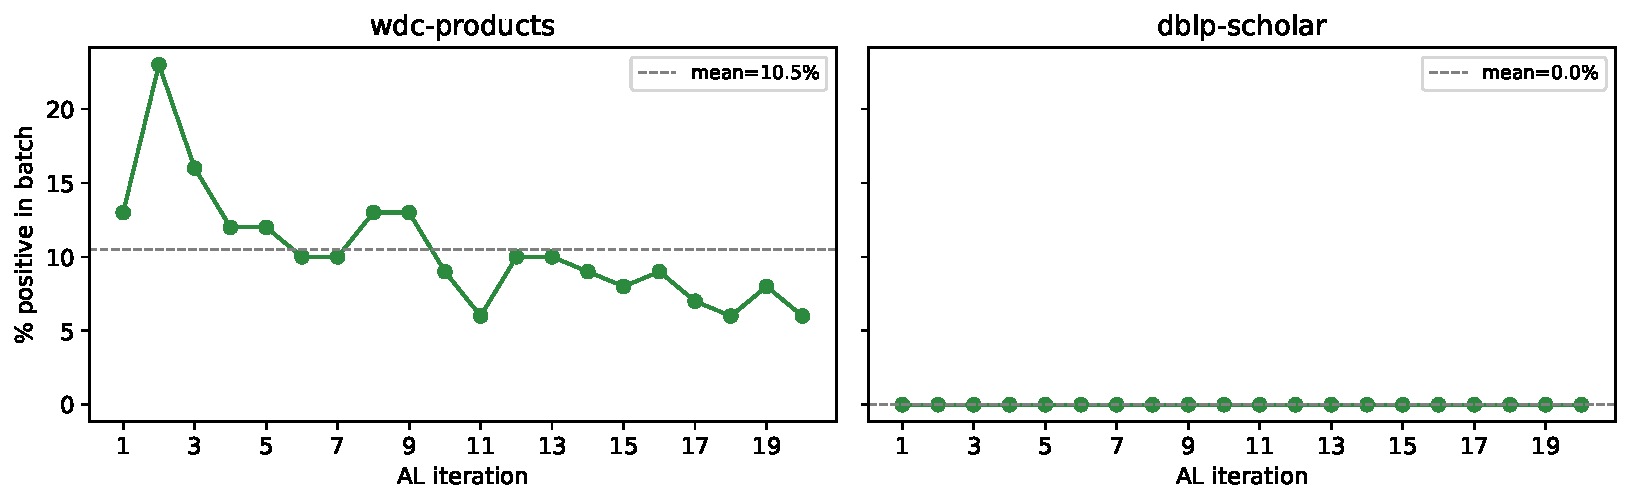
\includegraphics[width=\textwidth]{figures/al_positive_rate.pdf}
  \caption{Share of positive teacher labels per active-learning iteration (100 pairs each). On WDC Products (left) the rate averages about 10\% and declines over the iterations; on DBLP-Scholar (right) not a single positive is found among 2{,}000 labeled pairs. This is the positive-scarcity result of Section~\ref{sec:method_llm_filter} in one picture.}
  \label{fig:al_positive_rate}
\end{figure}

\section{Strategy 3: Web Retrieval Augmentation}
\label{sec:method_web}

The third strategy attacks the limitation that the first two cannot escape: everything so far recombines or perturbs records the benchmark already contains. Web retrieval brings in \emph{new} records from outside. The idea is simple: for a product in the training set, other shops publish offers for the same product with different wording; for a paper, other bibliographic sites publish variant records. Retrieving such documents and pairing them with the original entity yields pairs whose positive side genuinely adds information. The pipeline has four steps.

\subsection{Step 1: Entity Sampling}
\label{sec:method_web_sampling}

Labeling budget is limited, so we do not retrieve for every training entity. Per dataset, 150 entities are sampled from each side (300 total), stratified to protect diversity: entities are grouped into buckets by \texttt{brand} (WDC Products) or \texttt{venue} (DBLP-Scholar), and no bucket may contribute more than 15\% of a side's sample. Sampling is restricted to training entities (Section~\ref{sec:method_disjoint}). For each sampled entity, a search query is built from its identifying attributes --- brand and title for products, title and authors for papers --- and truncated to 400 characters.

\subsection{Step 2: Web Search}
\label{sec:method_web_search}

Each query is sent to the Tavily search API,\footnote{\url{https://tavily.com}} requesting up to 5 results with basic search depth. Each result consists of a page title, URL, and a content snippet. The top 3 results per entity are passed to the next step; snippets are truncated to 800 characters.

\subsection{Step 3: Extraction and Labeling}
\label{sec:method_web_extract}

Raw web snippets are not records, so the teacher performs three subtasks in a single prompt (Appendix~\ref{app:prompts}): (1) decide whether the snippet describes a \emph{specific} product or paper at all --- category pages, blog posts, and search-result pages are marked irrelevant and discarded; (2) if relevant, extract a structured record with exactly the benchmark's attribute schema, using empty strings for attributes the snippet does not mention; (3) decide whether the extracted record matches the original entity, using the same match definition and decisive-attribute instructions as in Strategy~2. The output is a pair (original record, extracted web record) with a teacher label.

This step is where the strategy's characteristic bias enters. Because the query is built from the entity's own brand and title, the search engine mostly returns pages about \emph{that product} --- which is the point, but it means the harvested pairs are predominantly positives. The relevant slice for WDC Products came out at 81\% positive. This skew is inherent to retrieval by identity ---
searching for a product finds that product --- and Chapter~\ref{ch:iteration} describes a follow-up experiment that tried to engineer the complementary hard negatives deliberately.

\subsection{Step 4: Finalization}
\label{sec:method_web_finalize}

The relevant labeled pairs are serialized into the benchmark schema and appended to the original training set. For WDC Products this added 803 pairs (yielding 3{,}303 total, 34.8\% positive); for DBLP-Scholar, 742 pairs (17{,}965 total, 21.4\% positive). Before training, a random sample of the labeled pairs was manually reviewed for label noise; the labels were found to be plausible, with the caveat that web snippets are sometimes too thin to decide variant-level questions with certainty.

Web retrieval is the only strategy of the three that adds new positive \emph{entities} --- new descriptions of training products from other shops --- and is therefore the only one that addresses the positive-scarcity problem of Strategy~2 head-on. Its weakness is textual: extracted web records are written differently from the benchmark's records (marketing copy, truncated snippets, missing attributes), so the added pairs are of type (benchmark record, web record) while the test set consists purely of (benchmark record, benchmark record) pairs. The consequences of this distribution mismatch surface in Chapters~\ref{ch:results} and~\ref{ch:iteration}.

\section{Ensuring Entity-Disjoint Augmentation}
\label{sec:method_disjoint}

All three pipelines share one hygiene rule: \textbf{augmentation may only use entities from the training split.} String augmentation satisfies it trivially, since it only rewrites existing training pairs. The LLM and web pipelines had to be made to satisfy it --- and were not in their first version.

The first version of the blocking step (Section~\ref{sec:method_llm_blocking}) built its candidate pool over the \emph{full} entity tables and excluded only known \emph{pairs}, on the reasoning that no benchmark pair would then be duplicated. That reasoning misses the point of entity-disjointness. The WDC Products entity tables contain about 2{,}900 entities per side, of which only about 1{,}000 appear in training; the rest are validation and test entities. Blocking over all of them meant that 59\% of the added LLM pairs on WDC Products (and 78\% on DBLP-Scholar) contained at least one held-out entity, with teacher labels attached. No exact test pair was leaked, but the student saw the \emph{text} of test entities during training --- on a benchmark whose test set is specifically constructed from unseen entities. The web pipeline had the analogous flaw in its entity sampling. An independent methodology audit caught the problem after the first full round of results.

The fix has three parts. First, a single module now serves as the authoritative source of entity-to-split membership, handling a subtlety that makes an ad-hoc fix dangerous: WDC Products uses one shared ID space (the same entity may appear on either side of a pair, so an excluded entity must be filtered from both sides), while DBLP-Scholar uses two separate per-side ID spaces whose numeric IDs overlap (so filtering must be side-specific, or a DBLP ID would wrongly exclude an unrelated Scholar record). Second, both pipelines filter their pools through this module: a candidate pair survives only if both entities belong to the training split. Third, a verification script recounts, for every augmented training file, how many pairs touch a held-out entity --- an entity appearing in validation or test but \emph{not} in training. The pass criterion is zero, and the final regenerated training sets meet it on both datasets. On WDC Products, whose benchmark splits are entity-disjoint, the augmented sets are therefore fully test-disjoint. On DBLP-Scholar, where most test entities also appear in training (Section~\ref{sec:data_hygiene}), the policy yields augmentation that is exactly as disjoint as the baseline itself --- it introduces no entity the original training set did not already use, which is the strongest guarantee possible on a non-disjoint benchmark.

The cost of honesty was substantial and is a finding in itself. All LLM-pipeline and web-pipeline data was regenerated on the clean pools, all affected models retrained, and the results re-evaluated. The clean WDC Products pool lost most of its positives (the leaked version had a healthy $\sim$25\% positive rate --- supplied, as it turned out, by held-out entities pairing with their training-set counterparts), and the clean DBLP-Scholar pool lost all of them. Every number reported in this thesis comes from the clean, regenerated data; where the contrast with the leaked version is instructive, it is reported explicitly and labeled as such.

% =====================================================================
\chapter{Experimental Setup}
\label{ch:setup}
% =====================================================================

This chapter fixes everything that is held constant across experiments: the training configuration of the student (Section~\ref{sec:setup_training}), the metrics (Section~\ref{sec:setup_metrics}), the multi-seed protocol (Section~\ref{sec:setup_seeds}), the statistical tests (Section~\ref{sec:setup_significance}), the three-layer evaluation scheme (Section~\ref{sec:setup_layers}), and the teacher-quality measurement (Section~\ref{sec:setup_teacher}).

\section{Training Configuration}
\label{sec:setup_training}

Every student is a \texttt{roberta-base} model fine-tuned for up to 10 epochs with batch size 8 and gradient accumulation over 4 steps (effective batch size 32), maximum sequence length 256, AdamW with weight decay 0.01, and 100 warmup steps. After each epoch the model is evaluated on the benchmark's validation split; the checkpoint with the best validation F1 is kept, and training stops early if validation F1 does not improve for 3 consecutive epochs. WDC Products students use the class-weighted loss of Section~\ref{sec:method_student}; DBLP-Scholar students use plain cross-entropy.

The learning rate needs a word of explanation. The initial single-seed experiments used $5 \cdot 10^{-5}$. During the multi-seed reruns, this rate occasionally caused training collapse on the imbalanced augmented sets (the student degenerating to the majority class), so the final protocol uses $2 \cdot 10^{-5}$ for all runs. All headline results in this thesis come from the $2 \cdot 10^{-5}$, three-seed protocol. Where earlier single-seed numbers at $5 \cdot 10^{-5}$ are mentioned for contrast, the learning-rate difference is acknowledged as a confound: the ``single-seed vs.\ multi-seed'' comparisons in this thesis bundle a seed change with a learning-rate change, and we do not attribute the differences to seed variance alone.

At evaluation time, the trained student predicts on the test split with the default argmax decision rule (equivalent to a 0.5 threshold on the match probability); Section~\ref{sec:results_threshold} examines threshold calibration separately. Per-pair predictions and match scores are saved for every run, which enables the paired tests and error analyses described below --- and allows every reported number to be recomputed from the stored predictions.

\section{Metrics}
\label{sec:setup_metrics}

The headline metric is F1 on the positive (match) class, with precision and recall reported alongside (Section~\ref{sec:preliminaries}). We do not use accuracy as a headline metric: with test positive rates of 11--19\%, accuracy is dominated by the majority class, and a matcher that rejects everything would already reach 0.89 accuracy on WDC Products. F1 is also what both comparison systems report \cite{zeakis2026distiller,steiner2026labeling}, which keeps Chapter~\ref{ch:comparison} on one scale.

\section{Multi-Seed Protocol}
\label{sec:setup_seeds}

Fine-tuning a 125M-parameter model on a few thousand pairs is noisy: different random seeds change weight initialization of the classification head and data ordering, and with them the final F1. The first round of experiments in this thesis used a single seed, and several of its conclusions --- including a statistically significant improvement of one strategy and a significant degradation of another --- turned out to be artifacts of that seed (Section~\ref{sec:results_seeds}). The final protocol therefore trains every configuration three times with seeds 13, 42, and 87, and reports F1 as mean $\pm$ standard deviation across seeds. The standard deviation is the sample estimator (dividing by $n{-}1$), matching how \citet{steiner2026labeling} and DistillER report variation across runs; with $n{=}3$ the estimate is coarse, but it reliably reveals when a delta between two configurations is smaller than the run-to-run noise of either.

Three seeds are a compromise dictated by compute (each configuration is a full fine-tuning run), and they set the resolution limit of the study: on WDC Products the observed seed noise is $\pm 0.015$--$0.020$ F1, so mean differences below roughly 0.02 cannot be distinguished from noise at this sample size. Claims in this thesis are phrased accordingly --- ``no detectable effect at $n{=}3$'' rather than ``no effect''.

\section{Statistical Significance Testing}
\label{sec:setup_significance}

Whenever two students are compared, both are evaluated on the \emph{same} test pairs, so the comparison is paired. Unpaired tests (such as the two-proportion $z$-test on accuracy) throw away the pairing and are the wrong tool; an earlier version of our analysis used one, and switching to the correct paired test changed two conclusions on DBLP-Scholar. Following \citet{dietterich1998approximate}, model-versus-model comparisons use \textbf{McNemar's test} \cite{mcnemar1947note} on the discordant pairs --- test items that exactly one of the two models classifies correctly --- with the exact two-sided binomial p-value.

McNemar's test operates on binary correctness, not on F1. To quantify uncertainty on F1 itself we additionally report a \textbf{paired bootstrap} \cite{efron1994introduction}: test pairs are resampled with replacement 10{,}000 times, the same resampled indices are applied to both models to preserve pairing, and a percentile confidence interval is computed for each model's F1 and for the F1 difference. As an effect size we report \textbf{Cohen's $h$} on accuracy \cite{cohen1988statistical}, so that statistical significance is always accompanied by a measure of practical significance --- with test sets of 4{,}500--5{,}742 pairs, tiny effects can be significant.

Because the multi-seed protocol produces three prediction sets per configuration, the paired tests are run on \emph{seed-averaged predictions}: the per-pair match scores of the three seeds are averaged and thresholded at 0.5, and McNemar's test compares these ensemble predictions. To be precise about what this tests: it compares the score-averaged ensembles of the two configurations, not the distribution of per-seed results; with $n{=}3$ seeds, a test across seeds would have essentially no power, and the ensemble comparison is the practical alternative. Finally, the thesis runs roughly a dozen such comparisons at $\alpha = 0.05$; under a Bonferroni correction \cite{dunn1961multiple} the threshold becomes $\approx 0.004$, and we mark which of the significant results survive it. Only one does.

\section{Three-Layer Evaluation Scheme}
\label{sec:setup_layers}

Downstream F1 alone cannot explain \emph{why} a strategy helps or fails, so every strategy is evaluated on three layers:

\begin{enumerate}
\item \textbf{Standard metrics:} precision, recall, F1 of the student on the test split, under the protocol above.
\item \textbf{Training set characteristics:} properties of the expanded training file itself --- size, positive rate, corner-case proportion, coverage of decisive attributes (WDC Products), and pairwise overlap between the pairs added by different strategies. Corner cases are defined via token-level Jaccard similarity between the two records (computed on value tokens, with serialization markers stripped): a \emph{hard positive} is a match with similarity below 0.3, a \emph{hard negative} a non-match with similarity above 0.4. The asymmetric thresholds reflect the asymmetry of the two error types: matches routinely share many tokens, so a match only becomes hard when overlap is very low, whereas a non-match becomes confusable already at moderate overlap. The middle band (0.3--0.4) is deliberately left neutral. These thresholds are heuristic; they are used consistently across all strategies and datasets, so comparisons between strategies are on equal footing even if the absolute corner-case percentages shift with the threshold choice.
\item \textbf{Qualitative error analysis:} misclassified test pairs of each student are grouped into four classes --- highly similar non-matches (false positives with similarity $> 0.5$), dissimilar matches (false negatives with similarity $< 0.2$), noisy or incomplete records (one side shorter than six value tokens), and the remaining ambiguous variant cases --- with counts and representative examples per class.
\end{enumerate}

The second layer directly checks the design requirements of Section~\ref{sec:method_requirements}; the third shows where each student actually fails and whether the failure profile changes with the training set.

\section{Measuring Teacher Label Quality}
\label{sec:setup_teacher}

The design requirements demand low teacher label noise, and ``low'' should be a number, not an impression. For WDC Products this can be measured exactly: the benchmark's cluster ground truth determines the true label of \emph{any} pair of its entities --- including the new pairs our pipelines created, which the benchmark never labeled explicitly. We therefore score every teacher-labeled pair from the LLM pipeline (100 seed + 2{,}000 active-learning labels) against the cluster ground truth and report the teacher's accuracy, precision, recall, and F1, overall and per pipeline stage. The pipeline itself never sees the cluster IDs; they are used only for this audit. For DBLP-Scholar no per-entity ground truth exists for new pairs, so teacher quality there rests on the manual spot checks mentioned in Section~\ref{sec:method_web_finalize}.

% =====================================================================
\chapter{Results}
\label{ch:results}
% =====================================================================

This chapter reports the main experimental results. Section~\ref{sec:results_baseline} establishes the baselines and examines the WDC Products threshold question. Section~\ref{sec:results_main} presents the downstream results of the three expansion strategies (Layer 1). Section~\ref{sec:results_seeds} documents how the multi-seed protocol overturned earlier single-seed conclusions. Sections~\ref{sec:results_layer2} and~\ref{sec:results_teacher} analyze the expanded training sets and the teacher's label quality, and Section~\ref{sec:results_layer3} presents the error analysis (Layer 3). Section~\ref{sec:results_summary} condenses the chapter into its main findings.

\section{Baselines}
\label{sec:results_baseline}

Table~\ref{tab:baselines} shows the baseline students trained on the unmodified training sets. On DBLP-Scholar, \texttt{roberta-base} reaches an F1 of 0.9559 $\pm$ 0.0019 --- the expected near-ceiling result for a transformer on this benchmark, with the memorization caveat from Section~\ref{sec:data_hygiene}. On WDC Products the class-weighted baseline reaches 0.659 $\pm$ 0.015; the run-to-run spread is an order of magnitude larger than on DBLP-Scholar (per-seed F1: 0.677, 0.649, 0.653), which quantifies how unstable small-data fine-tuning is on this benchmark and why single-seed comparisons on it are unreliable.

\begin{table}[tb]
  \centering
  \begin{tabular}{llccc}
    \toprule
    \textbf{Dataset} & \textbf{Run} & \textbf{Precision} & \textbf{Recall} & \textbf{F1} \\
    \midrule
    WDC Products & baseline (class-weighted) & 0.618 $\pm$ 0.056 & 0.715 $\pm$ 0.070 & 0.659 $\pm$ 0.015 \\
    DBLP-Scholar & baseline & 0.952 $\pm$ 0.004 & 0.960 $\pm$ 0.001 & 0.9559 $\pm$ 0.0019 \\
    \bottomrule
  \end{tabular}
  \caption{Baseline students (3-seed mean $\pm$ sample standard deviation, seeds 13/42/87).}
  \label{tab:baselines}
\end{table}

\subsection{The WDC Products Ceiling and the Prior Shift}
\label{sec:results_threshold}

Our WDC Products baseline sits below the 0.70--0.80 range that Ditto reports on its product benchmarks \cite{li2020deep}. Part of the explanation is the deliberately hard 80\%-corner-case configuration and the small training size, but a second, less obvious part is the prior shift documented in Section~\ref{sec:data_hygiene}: the student is trained, validated, and early-stopped against a 20\% positive rate, then tested against 11.1\%. A model calibrated to the training prior will over-predict matches on the test set at the default threshold.

To quantify how much of the gap the decision threshold could recover, we calibrated the threshold of the class-weighted baseline in four ways (single-seed analysis; Appendix~\ref{app:threshold} gives the full table). The default argmax rule yields F1 0.641. Tuning the threshold for maximum F1 on the \emph{validation} split makes things slightly worse (0.632 at threshold 0.444) --- validation mirrors the training prior, not the test prior, so it pulls the threshold in the wrong direction. Matching the threshold to the known test prior costs even more (0.565). The oracle threshold --- tuned directly on the test set, an upper bound no fair method can reach --- is far above the default (0.843) and yields 0.659, a gain of just +0.018. The conclusion is twofold: the model indeed over-predicts positives at the default cut, confirming the prior-shift diagnosis, but no legitimately selectable threshold recovers more than a fraction of the gap. The WDC Products ceiling of roughly 0.64--0.68 in our setting is thus substantially a property of the benchmark configuration, and we evaluate all strategies at the common default threshold.

\section{Downstream Results of the Three Strategies}
\label{sec:results_main}

Tables~\ref{tab:results_wdc} and~\ref{tab:results_dblp} present the headline results: the three expansion strategies against the baseline, per dataset, under the full protocol of Chapter~\ref{ch:setup} (three seeds, McNemar on seed-averaged predictions, paired bootstrap on F1). Figure~\ref{fig:results_bars} shows the same picture graphically, together with the second-iteration configurations that Chapter~\ref{ch:iteration} discusses; the visual message is that every error bar overlaps the baseline's on WDC Products, while on DBLP-Scholar the differences are barely visible at all.

\begin{figure}[tb]
  \centering
  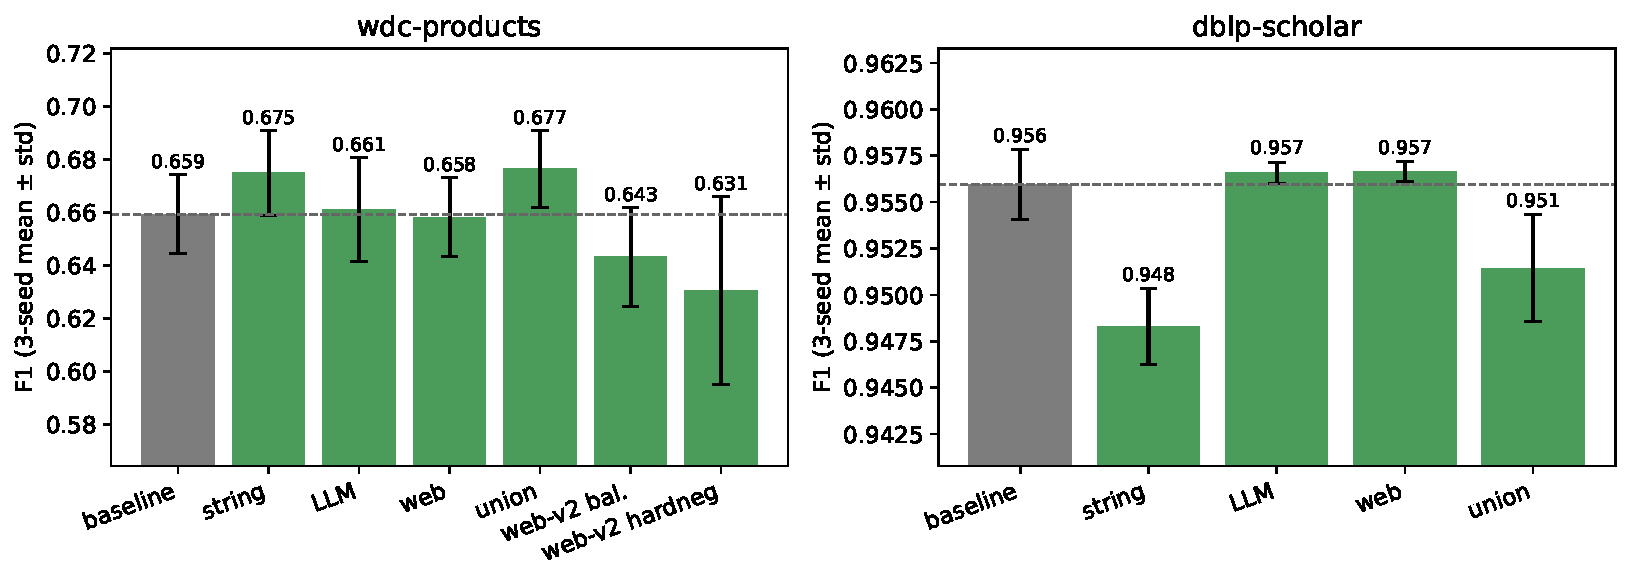
\includegraphics[width=\textwidth]{figures/results_f1_bars.pdf}
  \caption{Test F1 of all evaluated configurations (3-seed mean $\pm$ sample std). The dashed line marks the baseline mean. Left: WDC Products (class-weighted runs), including the union and web-v2 variants of Chapter~\ref{ch:iteration}. Right: DBLP-Scholar. No configuration separates from the baseline by more than the seed noise except the web-v2 variants, which are significantly worse.}
  \label{fig:results_bars}
\end{figure}

\begin{table}[tb]
  \centering
  \begin{tabular}{lcccrl}
    \toprule
    \textbf{Run} & \textbf{Precision} & \textbf{Recall} & \textbf{F1} & \textbf{$\Delta$F1} & \textbf{McNemar $p$} \\
    \midrule
    baseline & 0.618 $\pm$ 0.056 & 0.715 $\pm$ 0.070 & 0.659 $\pm$ 0.015 & --- & --- \\
    string\_aug & 0.618 $\pm$ 0.051 & 0.751 $\pm$ 0.068 & \textbf{0.675 $\pm$ 0.016} & +0.016 & 0.244 (n.s.) \\
    llm\_aug & 0.587 $\pm$ 0.031 & 0.759 $\pm$ 0.050 & 0.661 $\pm$ 0.020 & +0.002 & 0.356 (n.s.) \\
    web\_aug & 0.589 $\pm$ 0.043 & 0.750 $\pm$ 0.035 & 0.658 $\pm$ 0.015 & $-$0.001 & 0.396 (n.s.) \\
    \bottomrule
  \end{tabular}
  \caption{WDC Products test results (3-seed mean $\pm$ std; all runs class-weighted). No strategy differs significantly from the baseline.}
  \label{tab:results_wdc}
\end{table}

\begin{table}[tb]
  \centering
  \begin{tabular}{lcccrl}
    \toprule
    \textbf{Run} & \textbf{Precision} & \textbf{Recall} & \textbf{F1} & \textbf{$\Delta$F1} & \textbf{McNemar $p$} \\
    \midrule
    baseline & 0.952 $\pm$ 0.004 & 0.960 $\pm$ 0.001 & \textbf{0.9559 $\pm$ 0.0019} & --- & --- \\
    string\_aug & 0.927 $\pm$ 0.007 & 0.971 $\pm$ 0.005 & 0.9483 $\pm$ 0.0020 & $-$0.008 & 0.0079 (worse) \\
    llm\_aug & 0.953 $\pm$ 0.006 & 0.961 $\pm$ 0.006 & 0.9566 $\pm$ 0.0006 & +0.001 & 0.728 (n.s.) \\
    web\_aug & 0.948 $\pm$ 0.006 & 0.966 $\pm$ 0.007 & 0.9567 $\pm$ 0.0005 & +0.001 & 0.935 (n.s.) \\
    \bottomrule
  \end{tabular}
  \caption{DBLP-Scholar test results (3-seed mean $\pm$ std). Only string augmentation differs significantly from the baseline --- it is worse; the effect is nominal under Bonferroni correction.}
  \label{tab:results_dblp}
\end{table}

\textbf{On WDC Products, no strategy beats the baseline.} String augmentation has the best mean (+0.016 F1) and wins on two of three seeds, but it loses on the third, its delta sits inside the $\pm$0.015--0.020 seed-noise band, and McNemar's test on the seed-averaged predictions is far from significance ($p = 0.244$). The LLM and web strategies land within $\pm$0.002 of the baseline --- statistical ties. Recall shifts upward under every augmentation (0.715 $\rightarrow$ 0.750--0.759) at the cost of precision, consistent with all three strategies exposing the student to more positive-region variation without teaching it the decisive distinctions that would protect precision.

\textbf{On DBLP-Scholar, the baseline is unbeaten, and one strategy reliably hurts.} String augmentation loses on all three seeds ($-$0.008 F1, $p = 0.0079$); the effect is tiny (Cohen's $h \approx 0.03$) and only nominal under Bonferroni correction, but its direction is consistent. The mechanism is visible in the precision--recall split: doubling the training set with perturbed copies pushes recall up (0.960 $\rightarrow$ 0.971) but costs more precision (0.952 $\rightarrow$ 0.927), a bad trade on a dataset where the baseline's errors are already concentrated in a thin band of genuinely ambiguous pairs (Section~\ref{sec:results_layer3}). Perturbation noise near the ceiling erases signal rather than adding robustness --- some perturbed copies of hard negatives lose exactly the tokens that made them negatives (the risk anticipated in Section~\ref{sec:method_string}). The LLM and web strategies tie the baseline ($p = 0.73$ and $0.94$): 2{,}085 clean teacher-labeled hard negatives (LLM) and 742 web pairs changed nothing measurable.

Answering RQ1--RQ3 directly: none of the three strategies improves the student at a level distinguishable from seed noise, on either dataset. The remainder of the thesis is about \emph{why} --- and the answer differs per strategy, which is what makes the negative result informative.

\section{What Multi-Seed Evaluation Changed}
\label{sec:results_seeds}

The first complete round of experiments used a single seed (42) at learning rate $5 \cdot 10^{-5}$, and its conclusions differed sharply from Table~\ref{tab:results_wdc}: WDC string augmentation appeared to deliver a large, highly significant gain (+0.035, $p < 0.001$), WDC LLM augmentation appeared significantly \emph{harmful} ($-$0.027, $p = 0.0004$), and DBLP-Scholar LLM augmentation also appeared significantly worse. Under the three-seed protocol, all three conclusions dissolved: the string gain shrank to a non-significant +0.016, and both apparent LLM degradations turned out to be seed-42 outliers --- over three seeds, LLM augmentation \emph{ties} the baseline on both datasets.

Two lessons follow. First, the WDC Products baseline itself varies by 0.028 F1 across our three seeds, so any single-seed delta below roughly $\pm$0.03 on this benchmark is uninterpretable --- and most reported augmentation effects in the literature are of exactly that size. Second, as flagged in Section~\ref{sec:setup_training}, our protocol change bundled the seed change with a learning-rate change, so we avoid attributing the flips to seed variance alone; the honest statement is that the initial conclusions were not robust to a reasonable change of training conditions, which is precisely what robustness protocols exist to detect.

\section{Training Set Characteristics (Layer 2)}
\label{sec:results_layer2}

\begin{table}[tb]
  \centering
  \begin{tabular}{llrrrrr}
    \toprule
    \textbf{Dataset} & \textbf{Training set} & \textbf{N} & \textbf{\% Pos.} & \textbf{Hard pos.} & \textbf{Hard neg.} & \textbf{\% Corner} \\
    \midrule
    WDC & baseline & 2{,}500 & 20.0 & 435 & 65 & 20.0 \\
        & string\_aug & 5{,}000 & 20.0 & 882 & 123 & 20.1 \\
        & llm\_aug & 4{,}600 & 15.6 & 595 & 211 & 17.5 \\
        & web\_aug & 3{,}303 & 34.8 & 980 & 66 & 31.7 \\
    \midrule
    DBLP & baseline & 17{,}223 & 18.6 & 200 & 344 & 3.2 \\
         & string\_aug & 34{,}446 & 18.6 & 935 & 567 & 4.4 \\
         & llm\_aug & 19{,}308 & 16.6 & 200 & 385 & 3.0 \\
         & web\_aug & 17{,}965 & 21.4 & 337 & 351 & 3.8 \\
    \bottomrule
  \end{tabular}
  \caption{Layer 2: composition of the expanded training sets. Corner cases: hard positive = match with token-Jaccard $< 0.3$; hard negative = non-match with token-Jaccard $> 0.4$.}
  \label{tab:layer2}
\end{table}

Table~\ref{tab:layer2} checks the expanded training sets against the design requirements of Section~\ref{sec:method_requirements}, and Figure~\ref{fig:layer2_hist} shows the underlying similarity distributions per training set, split by label, with the corner-case thresholds marked. The headline is that the two central targets were missed everywhere.

\begin{figure}[tb]
  \centering
  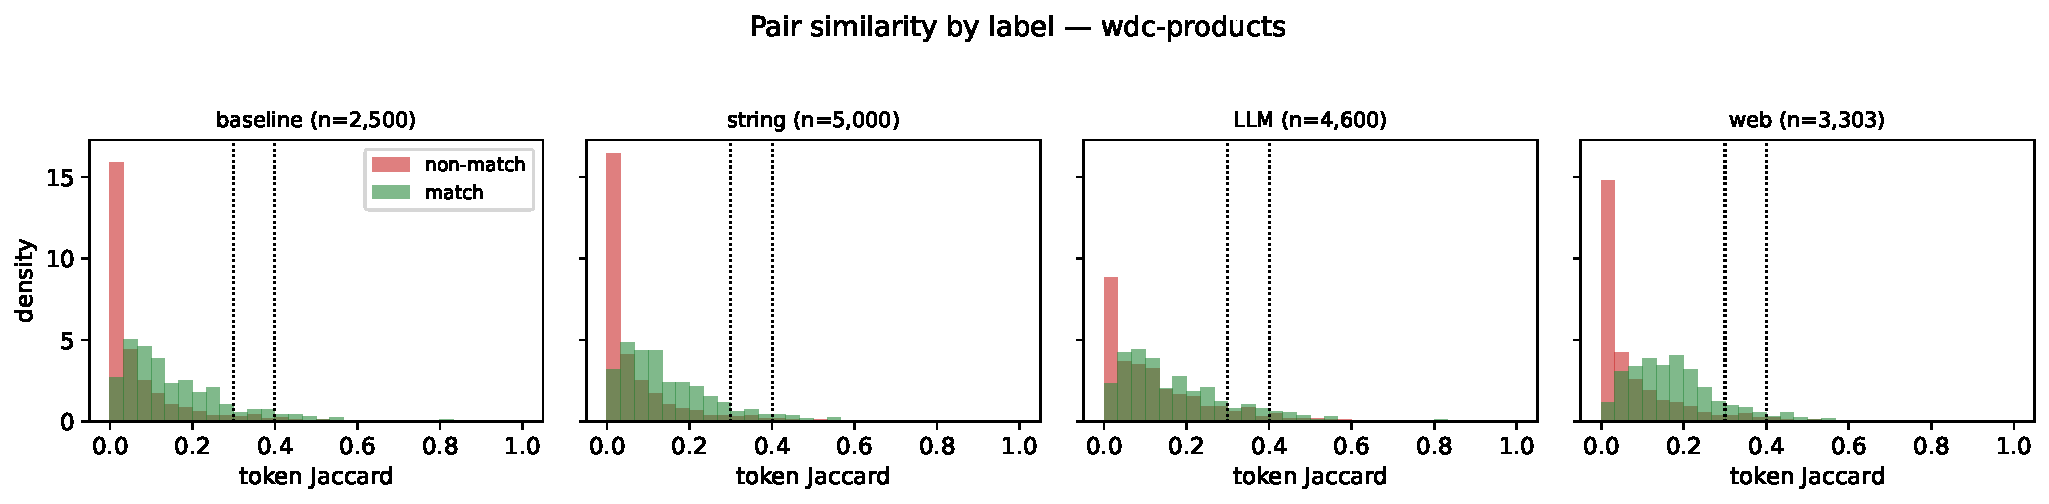
\includegraphics[width=\textwidth]{figures/layer2_sim_hist_wdc-products.pdf}\\[4pt]
  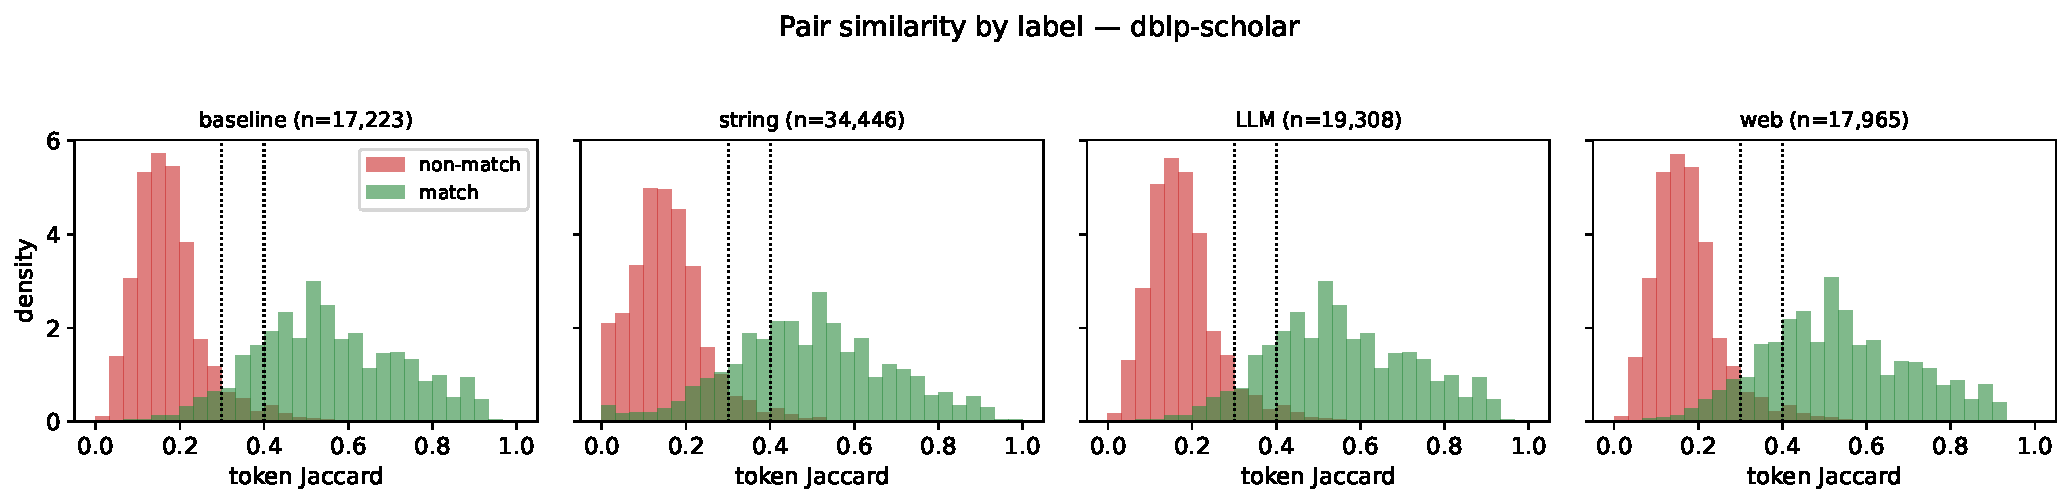
\includegraphics[width=\textwidth]{figures/layer2_sim_hist_dblp-scholar.pdf}
  \caption{Pair-similarity distributions (token-level Jaccard) of the four training sets, split by label; top row WDC Products, bottom row DBLP-Scholar. Dotted lines mark the corner-case thresholds (hard positive $< 0.3$, hard negative $> 0.4$). On WDC Products the match and non-match distributions overlap broadly --- the corner-case band is populated; on DBLP-Scholar they are almost perfectly separated, which is the visual form of the dataset's 3--4\% corner-case share.}
  \label{fig:layer2_hist}
\end{figure} The best corner-case proportion achieved on WDC Products is 31.7\% (web augmentation) against a target of 40--50\%; on DBLP-Scholar the best is 4.4\%, and no strategy even approaches the target. The positive-ratio picture is similarly mixed: LLM augmentation \emph{lowered} the positive rate on both datasets (to 15.6\% and 16.6\%), and web augmentation overshot on WDC Products (34.8\%).

Three per-strategy observations explain these numbers.

\textbf{LLM augmentation is positive-starved by construction.} As established in Section~\ref{sec:method_llm_filter}, the clean candidate pool contains almost no true matches (5.6\% on WDC Products, none discoverable on DBLP-Scholar), so the added slice is 10.3\% positive on WDC Products and 0\% positive on DBLP-Scholar. It does deliver one design goal: it is the only strategy that meaningfully increases \emph{hard negatives} on WDC Products (65 $\rightarrow$ 211), exactly what uncertainty sampling should find in a negative-dominated pool. For contrast, the leaked pre-fix version of this training set had a comfortable $\sim$25\% positive rate and 27.5\% corner cases --- numbers that met the targets and were entirely an artifact of held-out entities supplying the missing positives. The targets, in other words, were calibrated on what a leaky pipeline can achieve, and become structurally unreachable once the pipeline is honest.

\textbf{Web augmentation has the opposite skew.} Its added slice alone is 81\% positive (68\% corner cases) on WDC Products, diluted to 34.8\% only by the base training set, for the retrieval-by-identity reason given in Section~\ref{sec:method_web_extract}. It is also the only strategy whose hard-positive count rises sharply (980), since web descriptions of a training product often share few tokens with the benchmark's description of it.

\textbf{DBLP-Scholar structurally lacks corner cases.} Every strategy lands at 3--4\% corner cases on DBLP-Scholar, against 20--32\% on WDC Products. The bottom row of Figure~\ref{fig:layer2_hist} shows why: the match and non-match similarity distributions barely overlap. Paper records are either nearly identical (same paper) or clearly different (different papers); the borderline band that makes products hard barely exists --- title duplicates across genuinely different papers are rare. This single number goes a long way toward explaining both the 0.956 ceiling and the failure of every augmentation to move it.

Finally, the pairwise overlap between the added slices of the three strategies is exactly \textbf{zero} on both datasets --- no pair is produced by more than one strategy. String augmentation rewrites existing pairs, LLM augmentation pairs training entities in new combinations, and web augmentation imports external records, so they explore disjoint regions of pair space by construction. The three strategies are perfectly complementary in what they add, which motivates the union experiment of Section~\ref{sec:iter_union}: complementary additions can be combined without redundancy.

Attribute coverage (the remaining requirement) is stable: all strategies stay within a few points of the baseline's coverage of color ($\sim$35\%), memory/storage ($\sim$34--40\%), size ($\sim$37\%), bundle ($\sim$13\%), edition ($\sim$20\%), and model number ($\sim$30--35\%) mentions on WDC Products; the full table is in Appendix~\ref{app:coverage}. No strategy materially expands coverage of the underrepresented attributes --- none was designed to target attributes directly.

\section{Teacher Label Quality}
\label{sec:results_teacher}

Scoring all 2{,}100 teacher-labeled WDC Products pairs against the cluster ground truth (Section~\ref{sec:setup_teacher}) yields the following picture: accuracy \textbf{0.971}, precision 0.866, recall 0.858, F1 \textbf{0.862}, i.e.\ an overall label-noise rate of 2.9\% (29 false matches, 31 missed matches out of 2{,}100). Split by pipeline stage, the 100 similarity-ordered seed pairs were labeled with \emph{zero} errors, while the 2{,}000 uncertainty-selected active-learning pairs carry 3.0\% noise --- unsurprisingly, since uncertainty sampling deliberately routes the hardest pairs to the teacher.

Two conclusions follow. First, the teacher meets the low-noise design requirement: 97\% agreement with ground truth on adversarially selected pairs is a good annotator by any human-annotation standard. Second, and more importantly for interpreting the thesis, teacher noise is \emph{not} the bottleneck of LLM-based expansion. The teacher's labeling F1 (0.862) far exceeds the student's downstream F1 on this benchmark ($\sim$0.66); what the strategy lacked was not label quality but \emph{positives to label} (Section~\ref{sec:results_layer2}). This cleanly separates our negative result from the failure mode DistillER centers on --- noisy teachers --- and the point is taken up again in Chapter~\ref{ch:comparison}.

\section{Error Analysis (Layer 3)}
\label{sec:results_layer3}

The error analysis inspects the misclassified test pairs of each student under the classification scheme of Section~\ref{sec:setup_layers}. The counts reported in the text come from the initial single-seed runs (they predate the multi-seed protocol; the seed-42 LLM run among them was a low outlier), so we read this layer for failure \emph{mechanisms}, not for headline comparisons --- those are Table~\ref{tab:results_wdc} and~\ref{tab:results_dblp}. Figure~\ref{fig:error_classes} shows the class breakdown recomputed on the seed-averaged ensemble predictions of every run; the class profile is the same as in the single-seed analysis described below.

\begin{figure}[tb]
  \centering
  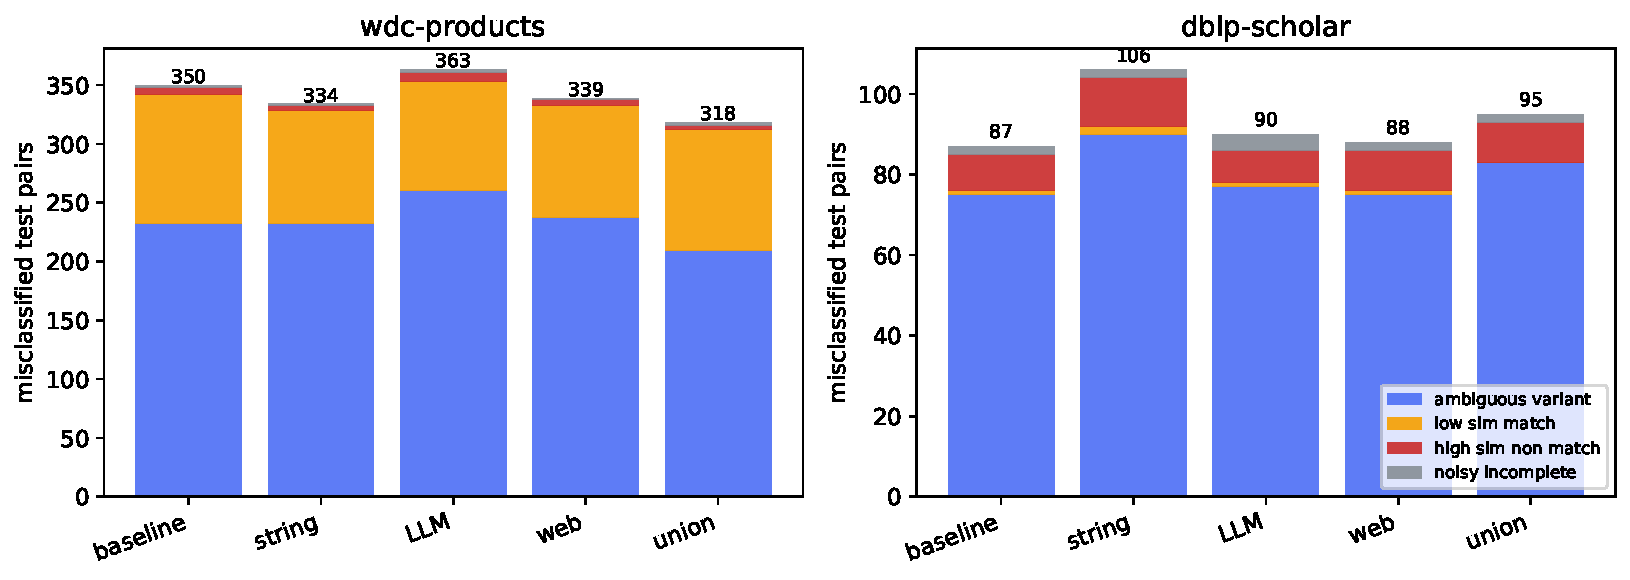
\includegraphics[width=\textwidth]{figures/layer3_error_classes.pdf}
  \caption{Misclassified test pairs per run, broken down into the four error classes of Section~\ref{sec:setup_layers} (computed on the seed-averaged ensemble predictions). The distribution is dominated by ambiguous variant cases on both datasets, and the profile barely changes across training sets --- augmentation shifted error counts, not error kinds.}
  \label{fig:error_classes}
\end{figure}

On \textbf{WDC Products}, errors are dominated by the \emph{ambiguous variant} class (62--78\% of errors across runs): pairs at moderate similarity where the student crossed the decision boundary in the wrong direction, typically product variants differing in one decisive attribute. A representative false positive pairs a Kingston A2000 NVMe SSD in 500\,GB against the same drive in 1{,}000\,GB: nearly all tokens agree, the capacity token decides, and the student weights it insufficiently. The second-largest class is dissimilar matches (19--36\%): the same product described so differently that token overlap gives the student almost nothing to hold on to. Classic high-similarity non-matches (e.g.\ a Corsair 570X case in white versus black) are rarer than expected (1--4\%) because the class-weighted student already handles many of them. Across training sets the \emph{profile} stays the same; augmentation shifted error \emph{counts}, not error \emph{kinds} --- consistent with the Layer 2 finding that no strategy substantially changed what the training data covers.

On \textbf{DBLP-Scholar}, students err on 1.6--2.0\% of test pairs, and the distribution is nearly invariant across all four training sets: 82--88\% ambiguous variants, plus a consistent handful (7--12 pairs) of a distinctive high-similarity non-match type --- the same paper title and authors at a conference and in a journal, distinguishable only by venue and year together. A representative example pairs ``Querying and Mining Data Streams: You Only Get One Look'' at SIGMOD 2002 against SIGMOD Record 2003: identical title, identical authors, different publication. This error type is exactly the hard-negative pattern that DBLP-Scholar's training data barely contains (Section~\ref{sec:results_layer2}), which motivated the targeted mining experiment of Section~\ref{sec:iter_hardneg}. The full per-run breakdown and further examples are given in Appendix~\ref{app:errors}.

\section{Summary of Findings}
\label{sec:results_summary}

\begin{enumerate}
\item No expansion strategy improves the student at a level distinguishable from seed noise, on either benchmark (RQ1--RQ3). String augmentation has the best WDC Products mean (+0.016, n.s.) and is the only strategy with a significant effect anywhere --- a tiny, consistent \emph{degradation} on DBLP-Scholar.
\item The design targets for the expanded training sets (25\% positive, 40--50\% corner cases) were not met by any strategy (RQ4). For LLM-based expansion this is structural: entity-disjoint pools on a closed benchmark contain almost no new positives, and the targets were only ever met by the leaked pipeline version.
\item The teacher is not the problem: 97.1\% label accuracy (F1 0.862) on adversarially selected pairs, with zero errors on the easier seed pairs.
\item The added slices of the three strategies overlap in zero pairs --- they are perfectly complementary, leaving union training as a natural follow-up.
\item Single-seed evaluation produced three conclusions (one significant gain, two significant losses) that did not survive the multi-seed protocol; WDC Products seed noise alone spans $\pm$0.02 F1.
\end{enumerate}

% =====================================================================
\chapter{Second Iteration: Targeted Improvements}
\label{ch:iteration}
% =====================================================================

After reviewing the first-round results, the supervisor requested a second experimental iteration built on what the analysis had revealed. Four work items resulted: mining the specific hard-negative type that DBLP-Scholar lacks (Section~\ref{sec:iter_hardneg}), fixing the skew of the web slice while injecting deliberately generated hard negatives on WDC Products (Section~\ref{sec:iter_webv2}), training on unions of the complementary augmentation sets (Section~\ref{sec:iter_union}), and testing whether augmentation helps more when the base training set is artificially shrunk (Section~\ref{sec:iter_lowresource}). The first three are complete --- two returned clear negative results, and the union produced the best WDC Products mean without separating from string augmentation alone; the low-resource ablation is still running at the time of writing.

\section{Hard-Negative Mining for DBLP-Scholar}
\label{sec:iter_hardneg}

The error analysis identified DBLP-Scholar's one distinctive hard error type: same title and authors, different publication (conference paper versus its journal version). The Layer 2 analysis showed the training data barely contains such pairs. The obvious intervention is to mine them directly: search the entity tables for record pairs with near-identical titles whose venue \emph{and} year both differ, keeping conference/journal cross-pairs and title duplicates as separate categories.

The mining returned \textbf{92} clean hard negatives --- 42 conference/journal cross-pairs and 50 title duplicates --- and this small count is itself the finding: 92 is not a sampling budget but the structural ceiling. DBLP-Scholar simply does not contain many same-title-different-paper cases, which explains both the near-zero hard-negative counts in Layer 2 and, in part, the F1 ceiling. Training with these 92 pairs added (single seed, since the expected effect is bounded by the handful of corresponding test errors) changed nothing: F1 0.9573 versus baseline 0.9579, McNemar $p = 1.0$. A definitive null on a ceiling dataset: even a perfectly targeted repair cannot help when the training data cannot supply more than a few dozen examples of the failure mode --- and the failure mode itself accounts for only 7--12 test errors.

\section{Rebalanced Web Augmentation with Generated Hard Negatives}
\label{sec:iter_webv2}

The web slice's 81\% positive skew (Section~\ref{sec:results_layer2}) was the most actionable defect in the first round, and the intervention had two parts, the second suggested by the supervisor. First, \emph{rebalance}: downsample the web positives so the added slice approaches the 1:3 target ratio. Second, \emph{generate hard negatives}: for each of the 300 sampled products, ask the teacher for the names of three real products that are \emph{similar but different} (e.g.\ the neighboring model in the same product line); retrieve offers for those distractor names via Tavily; have the teacher extract each offer and \emph{verify} it is truly a different product (the verification dropped 142 candidates that turned out to be the same product under another name --- the generation step is imperfect in exactly the way one would expect); and pair the original product's offer with the distractor offer as a labeled hard negative. This produced \textbf{1{,}290} verified hard negatives, and two training variants: a balanced one (added slice $\approx$ 1:3 positive) and a hard-negative-heavy one.

\begin{table}[tb]
  \centering
  \begin{tabular}{lccrl}
    \toprule
    \textbf{Run} & \textbf{F1 (3 seeds)} & \textbf{$\Delta$F1} & \textbf{McNemar $p$} & \textbf{Verdict} \\
    \midrule
    baseline & 0.659 $\pm$ 0.015 & --- & --- & --- \\
    web\_aug (v1) & 0.658 $\pm$ 0.015 & $-$0.001 & 0.396 & tie \\
    web\_v2 balanced & 0.643 $\pm$ 0.019 & $-$0.016 & 0.0098 & significantly worse \\
    web\_v2 hard-neg-heavy & 0.631 $\pm$ 0.036 & $-$0.029 & 0.0024 & significantly worse$^{*}$ \\
    \bottomrule
  \end{tabular}
  \caption{WDC Products: rebalanced web augmentation with generated hard negatives (3 seeds, class-weighted). $^{*}$Survives Bonferroni correction --- the only comparison in the thesis that does.}
  \label{tab:webv2}
\end{table}

The result (Table~\ref{tab:webv2}) is the opposite of the hypothesis: both variants are significantly \emph{worse} than the baseline, and the harder-negative-heavy variant is worse than the balanced one ($-$0.029, $p = 0.0024$, the only result in this thesis that survives Bonferroni correction). The error analysis on the seed-averaged predictions locates the damage precisely: false positives \emph{increased} from 216 (baseline) to 259 (balanced) to 283 (hard-neg-heavy), concentrated in the ambiguous-variant class. Adding verified hard \emph{negatives} made the student over-predict \emph{matches} more.

The mechanism, we argue, is the distribution mismatch anticipated in Section~\ref{sec:method_web_finalize}. Every generated hard negative is a pair (clean benchmark record, web-extracted offer), but the test set consists of (clean, clean) pairs. The student learns its decision boundary partly on web-styled text --- truncated snippets, marketing phrasing, sparse attributes --- and what it learns there does not transfer to benchmark-styled pairs; meanwhile the class-weighted loss over the remaining web positives and the off-distribution negatives pushes the boundary toward over-prediction on the clean data. The negatives themselves were verified to be high quality; the problem is not their labels but their \emph{text}. Together with the fact that LLM augmentation's clean, in-distribution hard negatives merely produced a tie (Table~\ref{tab:results_wdc}), the conclusion of this iteration is: \textbf{web augmentation's binding problem is the web-versus-benchmark text mismatch, not the positive ratio} --- fixing the ratio while deepening the mismatch made things strictly worse.

\section{Training on Unions of the Augmentation Sets}
\label{sec:iter_union}

The zero pairwise overlap between the three added slices (Section~\ref{sec:results_layer2}) raises a natural question the supervisor asked explicitly: if each strategy contributes different pairs, does their \emph{union} help where the parts did not? We built union training files on top of the shared base --- the full union (base + string + LLM + web additions, deduplicated) and all pairwise combinations --- and trained the full union under the standard three-seed protocol. The combined files are the largest training sets in the thesis: 7{,}900 pairs (23.6\% positive) on WDC Products and 37{,}187 pairs (18.9\% positive) on DBLP-Scholar, i.e.\ 3.2$\times$ and 2.2$\times$ the respective base sets.

\begin{table}[tb]
  \centering
  \begin{tabular}{llccrl}
    \toprule
    \textbf{Dataset} & \textbf{Run} & \textbf{N pairs} & \textbf{F1 (3 seeds)} & \textbf{$\Delta$F1} & \textbf{McNemar $p$} \\
    \midrule
    WDC & baseline & 2{,}500 & 0.659 $\pm$ 0.015 & --- & --- \\
        & string\_aug (best single) & 5{,}000 & 0.675 $\pm$ 0.016 & +0.016 & 0.244 (n.s.) \\
        & union all & 7{,}900 & \textbf{0.677 $\pm$ 0.015} & +0.017 & 0.0122 (nominal) \\
    \midrule
    DBLP & baseline & 17{,}223 & \textbf{0.9559 $\pm$ 0.0019} & --- & --- \\
         & union all & 37{,}187 & 0.9514 $\pm$ 0.0029 & $-$0.005 & 0.302 (n.s.) \\
    \bottomrule
  \end{tabular}
  \caption{Union of all three augmentation slices versus the baseline and the best single strategy (3 seeds; WDC Products runs class-weighted). The WDC Products union has the best mean of any configuration in the thesis but is statistically tied with string augmentation alone ($p = 0.214$); its nominal significance against the baseline does not survive Bonferroni correction.}
  \label{tab:union}
\end{table}

The results (Table~\ref{tab:union}) are a qualified null. On \textbf{WDC Products}, the full union reaches 0.677 $\pm$ 0.015 --- the best mean of any configuration in this thesis, and the only one whose McNemar test against the baseline drops below 0.05 ($p = 0.0122$). But three facts keep us from calling it a win. First, the p-value is nominal: with roughly a dozen comparisons in the thesis, the Bonferroni threshold is about 0.004, and 0.0122 does not clear it. Second, the union still loses to the baseline on one of three seeds, exactly like string augmentation. Third, and most tellingly, the union is statistically indistinguishable from string augmentation alone ($p = 0.214$, mean difference +0.002) --- adding the 2{,}100 LLM-labeled pairs and the 803 web pairs on top of the string copies moved the mean by two thousandths. The complementarity that the zero pair overlap promised does not materialize as complementary \emph{signal}: the union's effect is the string effect. Given this, we did not train the pairwise combinations; every one of them is bracketed between a component that does nothing on its own and a union that adds nothing beyond string.

On \textbf{DBLP-Scholar}, the union is worse than the baseline on all three seeds ($-$0.005, not significant), consistent with its composition: it inherits the reliably harmful string slice (Section~\ref{sec:results_main}) and dilutes it with two slices that individually did nothing.

The union experiment sharpens the thesis's central point. Even 5{,}400 additional WDC Products pairs from three sources with zero mutual overlap --- perturbed copies, teacher-labeled hard negatives, and genuinely new web records --- cannot outperform the cheapest of the three on its own. More pairs of the kinds that honest expansion can produce is not the binding constraint; the missing ingredient remains new in-distribution positives, which none of the three sources supplies (Section~\ref{sec:disc_mechanisms}).

\section{Low-Resource Ablation}
\label{sec:iter_lowresource}

The comparison with DistillER suggests a specific hypothesis: LLM-labeled data helps most when the base training set is too small to cover the common patterns --- DistillER operates at 10\% of entities, and its largest gain from teacher labels occurs on its sparsest product dataset. Our WDC Products base set of 2{,}500 pairs may simply already be past that point. The ablation shrinks the base training set to 50\% and 25\%, combines each reduced base with the LLM-augmented slice, and measures whether the augmentation benefit grows as the base shrinks --- the regime of Figure~4 of \citet{steiner2026labeling}, and the most likely place in this whole thesis for augmentation to finally show a positive effect.

\pending{Pending: low-resource ablation (100\%/50\%/25\% base training set, each with and without the LLM-labeled slice) on WDC Products, 3 seeds each. Results and discussion will be inserted here.}

% =====================================================================
\chapter{Comparison with DistillER and Steiner \& Bizer}
\label{ch:comparison}
% =====================================================================

Two recent works study the same underlying question as this thesis --- can an LLM teacher create training data for a small entity matching student? --- and reach considerably more optimistic conclusions. This chapter takes both apart in detail and reconciles the difference. Section~\ref{sec:comp_framework} fixes what can and cannot be compared. Sections~\ref{sec:comp_distiller} and~\ref{sec:comp_aaron} treat DistillER \cite{zeakis2026distiller} and \citet{steiner2026labeling} in turn, and Section~\ref{sec:comp_synthesis} draws the joint picture: the three studies do not contradict each other --- they measure different regimes of the same underlying trade-off, and placing them side by side reveals a boundary that none of them shows alone.

\section{What Is Comparable, and What Is Not}
\label{sec:comp_framework}

Three axes must be fixed before any numbers are put side by side, because each one silently shifts F1 by more than the effects under discussion.

\textbf{Task framing: replacement versus expansion.} Both comparison works study \emph{replacement}: the teacher labels (or relabels) pairs drawn from the benchmark's own pair universe, and the student trained on machine labels is compared against a student trained on the same pairs with human labels. The question is ``how much quality is lost by swapping the annotator?'' This thesis studies \emph{expansion}: the human-labeled training set is kept, and the teacher labels \emph{new} pairs that the benchmark does not contain. The question is ``how much quality is gained by adding machine-labeled data?'' The distinction sounds procedural but decides what the candidate pool can contain --- the central mechanism of Section~\ref{sec:comp_aaron_pool}.

\textbf{Training budget.} DistillER trains on pairs built from roughly 10\% of each dataset's entities --- a deliberately low-resource regime. \citet{steiner2026labeling} label at the full benchmark scale, e.g.\ around 16{,}000--20{,}000 WDC Products pairs. This thesis trains on the small WDC Products split (2{,}500 pairs) plus modest additions. Absolute F1 comparisons across these budgets are meaningless unless made budget-aware, as Section~\ref{sec:comp_aaron_budget} shows on a concrete case.

\textbf{Benchmark version.} All three works use a WDC Products variant and a DBLP-Scholar-style benchmark, but the variants differ: we and \citet{steiner2026labeling} use the hard 80\%-corner-case configuration with the \emph{unseen} (entity-disjoint) test set; DistillER's product datasets (Abt-Buy, Amazon-Google, Walmart-Amazon) are older Magellan benchmarks with non-disjoint splits. Metric and protocol, at least, agree everywhere: F1 on the match class, mean over three seeds (they use seeds \{42, 52, 62\}, we use \{13, 42, 87\}), and we adopt the convention of \citet{steiner2026labeling} that two results are comparable when their $\pm 1$ std intervals overlap.

\section{Comparison with DistillER}
\label{sec:comp_distiller}

\subsection{Their Approach}
\label{sec:comp_distiller_approach}

DistillER \cite{zeakis2026distiller} distills a Qwen-2.5 32B teacher into small students across eight benchmarks (D2--D9), spanning products, bibliographic data, and other domains. Given a low-resource pair budget (from ~10\% of entities), the teacher labels the pairs and the student --- S-MiniLM or RoBERTa --- is fine-tuned on the noisy labels; the control is the same student trained on ground-truth labels for the same pairs. They further compare unsupervised strategies for \emph{selecting} which pairs to label (ranking by blocking similarity emerging as the most reliable, approximately maintaining a 3:1 negative-to-positive ratio), and, for LLM students, supervised fine-tuning on teacher-generated \emph{explanations} rather than bare labels --- their best overall variant, though it targets a different student class than ours.

\subsection{Result Comparison}
\label{sec:comp_distiller_results}

Table~\ref{tab:comp_distiller} places DistillER's RoBERTa student next to our results on the two shared dimensions: the bibliographic near-ceiling regime and the hard product regime.

\begin{table}[tb]
  \centering
  \begin{tabular}{llcc}
    \toprule
    \textbf{Regime} & \textbf{Dataset} & \textbf{RoBERTa + GT labels} & \textbf{RoBERTa + LLM labels} \\
    \midrule
    \multirow{2}{*}{Bibliographic}
      & D9 DBLP/Scholar (DistillER) & 0.89 & 0.86 \\
      & DBLP-Scholar (this thesis) & 0.9559 $\pm$ 0.0019 & 0.9566 $\pm$ 0.0006$^{a}$ \\
    \midrule
    \multirow{4}{*}{Products}
      & D2 Abt-Buy (DistillER) & 0.78 & 0.75 \\
      & D3 Amazon-Google (DistillER) & 0.40 & 0.41 \\
      & D8 Walmart-Amazon (DistillER) & 0.44 & \textbf{0.57} \\
      & WDC Products (this thesis) & 0.659 $\pm$ 0.015 & 0.661 $\pm$ 0.020$^{a}$ \\
    \midrule
    & Mean over all 8 (DistillER) & 0.66 & \textbf{0.69} \\
    \bottomrule
  \end{tabular}
  \caption{DistillER (RoBERTa student, Qwen-2.5:32b teacher, $\sim$10\% of entities) versus this thesis. $^{a}$Our ``LLM labels'' column is the \emph{expansion} setting (GT base + LLM-labeled additions), not pure replacement; budgets and benchmark versions also differ (Section~\ref{sec:comp_framework}), so trends, not absolute values, are comparable.}
  \label{tab:comp_distiller}
\end{table}

Three trends align across the studies, and one deviation is informative.

\textbf{Bibliographic data: same direction, different absolute level.} On DBLP/Scholar-type data, LLM labels do not beat ground truth in either study (DistillER: 0.86 vs.\ 0.89; ours: statistical tie). Our absolute F1 is far higher (0.956 vs.\ 0.89) for a budget reason --- we train on the full 17{,}223-pair split, they on a 10\% low-resource subset --- which usefully brackets the dataset: even at a tenth of the data, RoBERTa reaches 0.89, and at full data it saturates near 0.956. Both studies conclude that on this benchmark there is little for an LLM teacher to add.

\textbf{Products are the hard domain, for the same reason.} DistillER's product datasets are their weakest across all methods, and their diagnosis --- shared tokens between non-matching entities overwhelming the subtle decisive difference, their example being Cat6 Ethernet cables of 5\,m versus 15\,m --- is precisely the dominant error class of our WDC Products students (the 500\,GB versus 1\,TB SSD of Section~\ref{sec:results_layer3}). Two teachers (Qwen, Claude), two benchmark families, one failure mode: variant-level distinctions are where both teachers and students struggle, which supports treating it as a property of the product-matching task rather than of any single model.

\textbf{Selection ratios agree.} DistillER's finding that ranking-based selection maintaining roughly 3:1 negatives-to-positives performs best independently corroborates the 1:3 design target of Section~\ref{sec:method_requirements} --- and thereby sharpens our negative result: the target itself is well-supported; what our setting lacked was any honest way to \emph{reach} it (Section~\ref{sec:results_layer2}).

\textbf{The Walmart-Amazon deviation points at the interesting regime.} D8 is the one case where LLM labels beat ground truth by a wide margin (0.44 $\rightarrow$ 0.57). It is also DistillER's most extreme low-resource case for a product dataset: the ground-truth-trained student is so data-starved that even noisy teacher labels add net signal. Our WDC Products base of 2{,}500 pairs appears to be past that starvation point --- the base set already covers the common patterns, so additional teacher-labeled pairs of the kind our pools could supply added nothing. This reading is testable, and Section~\ref{sec:iter_lowresource} tests it: shrink our base set toward DistillER's regime and see whether the augmentation benefit appears.

\textbf{What does not transfer.} DistillER's central variable is teacher noise (their teacher-student agreement analysis drives the paper); our teacher audit (Section~\ref{sec:results_teacher}) shows 2.9\% noise, low enough that noise plays almost no role in our results. Conversely, our central variable --- the positive content of an entity-disjoint candidate pool --- does not arise in their setting at all, because their pairs come from the benchmark's own pair universe with ground-truth positives included by construction. The two studies fail (and succeed) on orthogonal axes, which is exactly why the joint picture in Section~\ref{sec:comp_synthesis} is more informative than either alone.

\section{Comparison with Steiner \& Bizer}
\label{sec:comp_aaron}

\subsection{Their Approach}
\label{sec:comp_aaron_approach}

\citet{steiner2026labeling} ask whether LLM-labeled training data is ``fit for use'': they generate candidate pools over entity matching benchmarks (including the same WDC Products 80\%-corner-case benchmark with the unseen test set that we use, and DBLP-Scholar), have LLM teachers (GPT-based, among others) label pairs selected by several strategies, train students (Ditto/RoBERTa among them) on the machine-labeled data, and compare against students trained on the original human labels. Their selection strategies include an active-learning variant --- a committee of feature-based classifiers over string-similarity features, querying by disagreement --- that our Strategy 2 (Section~\ref{sec:method_llm}) implements step for step. This makes the comparison unusually direct: same student architecture, same benchmark and test set (for WDC Products), same selection algorithm, an LLM teacher on both sides --- and one deliberate difference in the candidate pool.

\subsection{The Pool Difference That Decides Everything}
\label{sec:comp_aaron_pool}

Their pools are built from the benchmark's pair universe and \emph{recover 99.56--99.92\% of the original positive pairs}; the teacher then relabels what the benchmark already knew. Our pipeline \emph{excludes} every known pair --- by design, since duplicating or relabeling existing training pairs is not expansion --- and what remains after the exclusion is the complement of the benchmark: 5.6\% positives on WDC Products, none discoverable on DBLP-Scholar (Section~\ref{sec:method_llm_filter}).

This single design choice explains the headline divergence between the two studies. In their setting, active learning selects from a pool with a healthy positive rate, the machine-labeled set has a usable class balance, and the student trained on it lands close to the human-label student --- LLM labeling works. In our setting, the same active-learning algorithm, the same features, and a demonstrably accurate teacher (Section~\ref{sec:results_teacher}) produce a near-all-negative addition, because the pool has nothing else to offer --- LLM \emph{expansion} stalls. Nothing failed in between; the two pools simply contain different things. In distillation terms: replacement lets the teacher transfer knowledge about pairs the benchmark curated, while expansion asks the teacher to create knowledge about pairs nobody curated --- and on a closed benchmark, the curatable matches are already taken. We regard making this asymmetry visible --- and measurable, via the pool-composition numbers --- as the main conceptual contribution of the thesis.

\subsection{Head-to-Head Numbers}
\label{sec:comp_aaron_results}

\begin{table}[tb]
  \centering
  \begin{tabular}{llcc}
    \toprule
    \textbf{Dataset} & \textbf{Quantity} & \textbf{This thesis} & \textbf{Steiner \& Bizer} \\
    \midrule
    \multirow{3}{*}{WDC Products}
      & human-label baseline & 0.659 $\pm$ 0.015 \ (2{,}500 pairs) & 0.719 \ ($\sim$16k pairs) \\
      & AL (ML) / llm\_aug & 0.661 $\pm$ 0.020 \ (tie, expansion) & 0.707 $\pm$ 0.004 \ (replacement) \\
      & best over strategies & 0.675 $\pm$ 0.016 \ (string, n.s.) & 0.722 \ (AL-Ditto) \\
    \midrule
    \multirow{2}{*}{DBLP-Scholar}
      & human-label baseline & 0.9559 $\pm$ 0.0019 & 0.956 \\
      & AL (ML) / llm\_aug & 0.9566 $\pm$ 0.0006 \ (tie) & 0.938 $\pm$ 0.004 \\
    \bottomrule
  \end{tabular}
  \caption{Head-to-head with \citet{steiner2026labeling} (Ditto/RoBERTa student). WDC Products: same benchmark and unseen test set, different training budget. ``AL (ML)'' is their feature-ensemble active-learning variant --- algorithmically the same selection as our llm\_aug.}
  \label{tab:comp_aaron}
\end{table}

Table~\ref{tab:comp_aaron} shows the alignment. On \textbf{DBLP-Scholar}, where both studies train at full benchmark scale, the human-label baselines are essentially identical (0.9559 vs.\ 0.956) --- a useful mutual validation of two independent implementations. Their machine-labeled AL variant lands \emph{below} the human baseline ($-$1.8 F1 points, at 0.938), while our expansion variant ties it (+0.001): replacement pays a small noise tax on a saturated dataset, while expansion adds nothing but also breaks nothing. Both studies agree on the substantive point: near the ceiling, an LLM teacher does not improve on human labels.

On \textbf{WDC Products} the raw numbers look contradictory --- their baseline 0.719 versus ours 0.659 --- until the budget axis is fixed. Figure~\ref{fig:comparison_bars} summarizes the ground-truth-versus-teacher-labels contrast across all three studies in one view.

\begin{figure}[tb]
  \centering
  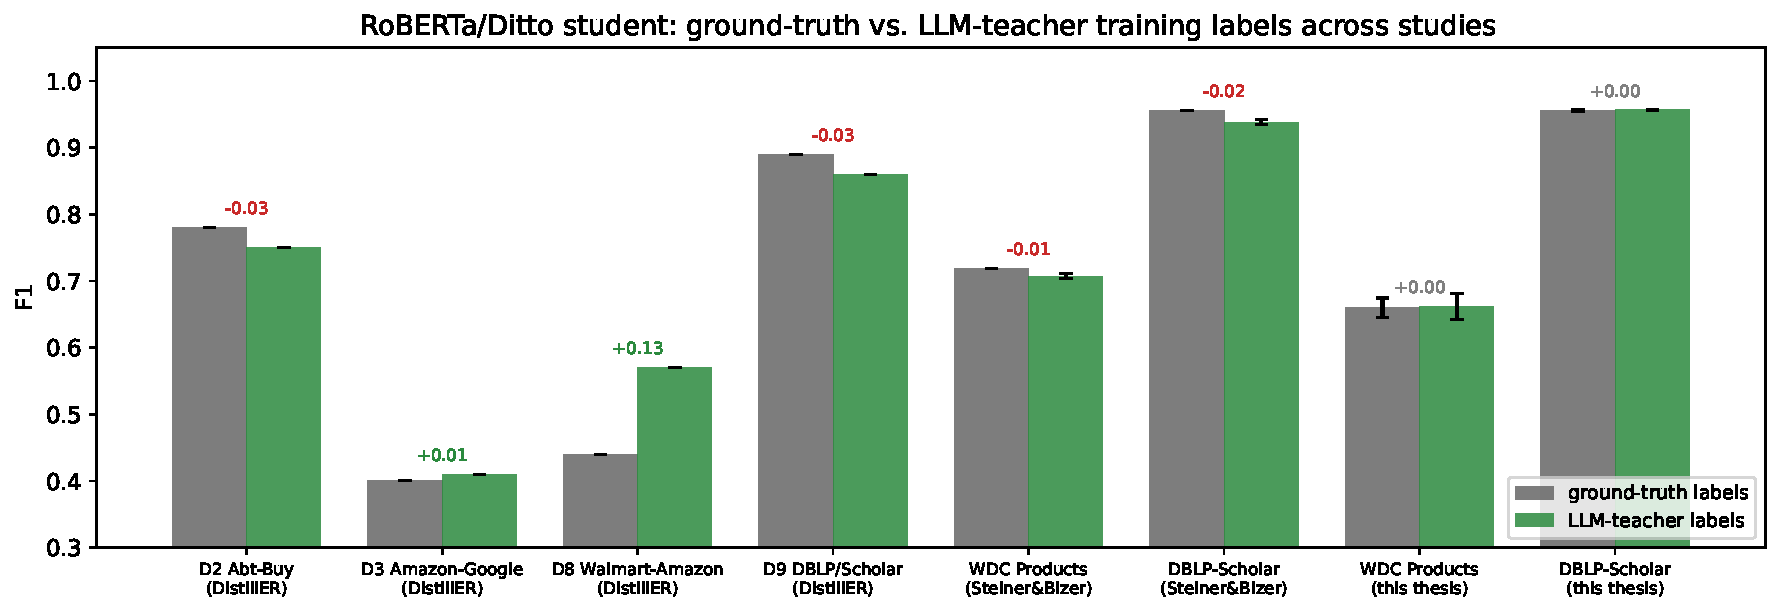
\includegraphics[width=\textwidth]{figures/comparison_gt_vs_llm.pdf}
  \caption{Students trained on ground-truth labels versus LLM-teacher labels across the three studies (RoBERTa/Ditto students; annotations give the delta). DistillER numbers from their Table 8 ($\sim$10\% of entities); Steiner \& Bizer numbers from their Table 1 (AL-ML variant); our bars are the expansion setting with 3-seed error bars. Budgets and benchmark versions differ between studies (Section~\ref{sec:comp_framework}), so the figure compares directions, not absolute levels: teacher labels help only in DistillER's most data-starved product case (Walmart-Amazon) and are roughly neutral or slightly harmful everywhere else.}
  \label{fig:comparison_bars}
\end{figure}

\subsection{A Budget-Aware Reading of the WDC Products Gap}
\label{sec:comp_aaron_budget}

The two baselines differ by exactly one variable: training size. They train on the large split ($\sim$16{,}000+ pairs); we train on the small split (2{,}500 pairs); benchmark, corner-case level, and unseen test set are identical. Their own learning curve (their Figure~4) shows WDC Products F1 rising from roughly 0.50 at 1{,}000 labeled pairs and only plateauing around 15{,}000--16{,}000 --- crossing 0.719 near the top. Figure~\ref{fig:budget_curve} places our configurations on this budget axis. Two consequences follow.

\begin{figure}[tb]
  \centering
  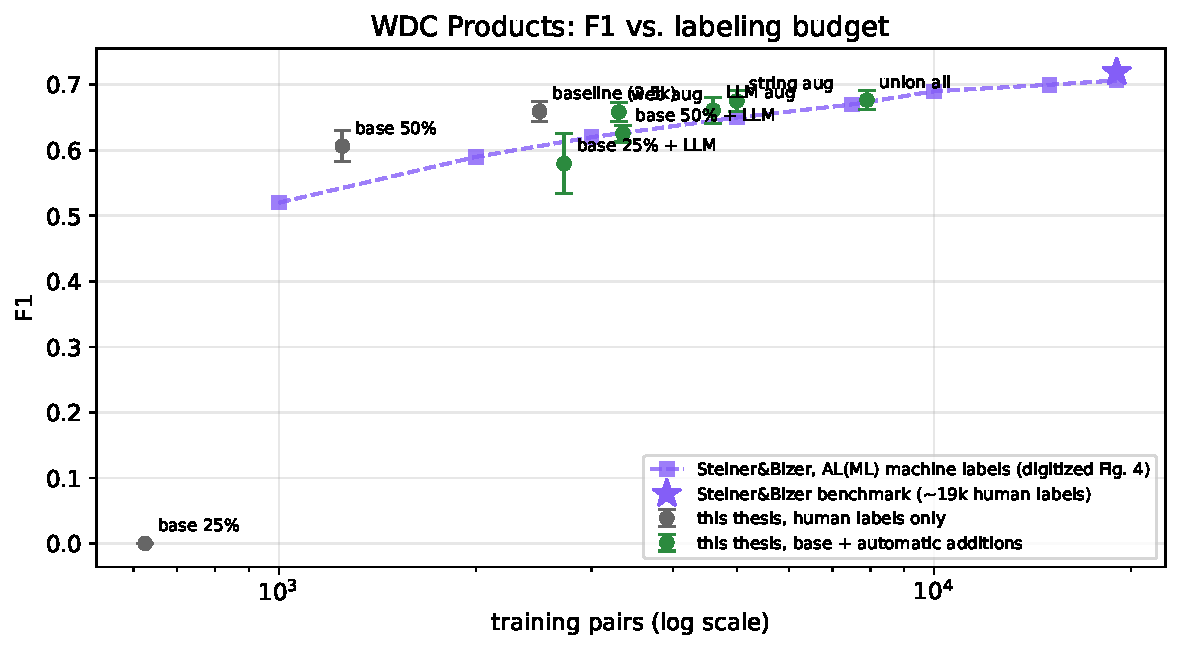
\includegraphics[width=0.85\textwidth]{figures/budget_curve_wdc.pdf}
  \caption{WDC Products F1 as a function of the number of training pairs (log scale). Purple: the machine-label learning curve of \citet{steiner2026labeling} (anchor points read approximately off their Figure~4; the star marks their large-split human-label benchmark). Gray/green with error bars: this thesis's configurations at their actual training sizes. Our human-label baseline at 2{,}500 pairs lies on their curve, and none of our expansions moves meaningfully up it --- growing the training set with expandable pairs is not equivalent to growing it with benchmark-quality labeled pairs.}
  \label{fig:budget_curve}
\end{figure}

First, the 0.06 baseline gap is fully explained by budget: 0.659 at 2{,}500 pairs is \emph{on} their curve, not below it. Second --- and this was the supervisor's original observation --- at a \emph{matched} budget of $\sim$2{,}500 labels, their machine-labeled student sits at roughly 0.55--0.62 on that same curve, i.e.\ \emph{below} our human-label baseline of 0.659. In other words: at our budget, 2{,}500 human labels beat 2{,}500 machine labels; machine labeling wins on cost only when it buys volume that humans cannot afford. That is their thesis, stated budget-aware --- machine labels are cheap enough to climb the curve --- and it coexists without contradiction with ours: at a fixed, already-labeled base, machine-labeled \emph{expansion} of a closed benchmark adds little, because the addable pairs are the wrong ones. The two studies describe the two ends of the same trade: \emph{scale} (their axis) versus \emph{marginal content} (ours).

\section{Synthesis}
\label{sec:comp_synthesis}

Placing the three studies side by side yields a consistent map of when LLM-teacher data helps a small entity matching student:

\begin{enumerate}
\item \textbf{Teacher quality is a solved sub-problem on these benchmarks.} DistillER's Qwen teacher, their GPT-class teachers, and our Claude teacher (97.1\% accuracy under adversarial selection) are all accurate enough that label noise is a secondary effect. None of the three studies' headline outcomes is driven by the teacher being wrong.
\item \textbf{What decides the outcome is what the teacher gets to label.} Replacement pools (both comparison works) contain the benchmark's positives; students trained on their machine labels approach human-label quality. Entity-disjoint expansion pools (this thesis) contain almost no undiscovered positives; the labeled addition is class-degenerate and the student does not move. The candidate pool, not the teacher or the student, is the binding constraint.
\item \textbf{Base-set saturation gates the benefit.} The one large machine-label win across all three studies (DistillER's Walmart-Amazon, +0.13) occurs at extreme data starvation; at our 2{,}500-pair base the effect is absent, and at full DBLP-Scholar scale everyone's effects vanish. LLM-teacher data behaves like a remedy for scarcity, not an amplifier of adequacy. (Section~\ref{sec:iter_lowresource} probes exactly this gate.)
\item \textbf{Product-variant distinctions remain the shared frontier.} All three studies bottom out on the same error type --- shared-token, single-attribute-difference product pairs --- regardless of teacher, student, or labeling regime. Progress here likely requires attribute-aware supervision rather than more pairs of the same kind.
\end{enumerate}

For a practitioner, the map reads: if you have almost no labels, let an LLM teacher label a similarity-ranked pool for you (DistillER's regime; strong evidence it works). If you can label the benchmark-scale pool, machine labels trade a point or two of F1 for a large cost saving (Steiner \& Bizer's regime). But if you already have a curated training set and hope an LLM will \emph{extend} it over the same entity universe --- this thesis's regime --- expect little: the extendable positives mostly do not exist, and importing them from outside (the web) runs into a text-distribution wall that naive retrieval does not cross.

% =====================================================================
\chapter{Discussion}
\label{ch:discussion}
% =====================================================================

\section{Three Mechanisms Behind the Negative Result}
\label{sec:disc_mechanisms}

The headline of this thesis --- automatic expansion did not improve the student --- would be uninteresting if it had a single cause or no cause. It has three, they are separable, and each was established by a different part of the evidence.

\textbf{Mechanism 1: positive scarcity in entity-disjoint pools.} A benchmark is, by construction, an attempt to enumerate the matches among its entities. Whatever match-finding process built the benchmark already harvested the discoverable positives into the labeled splits. An expansion pipeline that (correctly) excludes known pairs and (correctly) restricts itself to training entities therefore fishes in the leftovers: pairs that passed blocking similarity but were never labeled as matches --- overwhelmingly true negatives. We measured this directly: 5.6\% positives in the WDC Products pool, zero discoverable positives on DBLP-Scholar, and consequently a 10.3\%- and 0\%-positive added slice. No selection algorithm and no teacher can label positives that are not there. The practical formulation: \emph{on a closed benchmark, honest expansion is structurally positive-starved; the accessible new information is almost entirely negative}. Note the qualifier ``closed'' --- the mechanism is about benchmarks whose entity universe is fixed and pre-mined, which is exactly the situation of academic evaluation, and \emph{not} necessarily of production settings where new entities stream in continuously.

\textbf{Mechanism 2: text-distribution mismatch in web-imported data.} Web retrieval circumvents Mechanism 1 --- it demonstrably injected new positive records (81\% of its slice) --- and still failed, in the follow-up even significantly ($-$0.029 F1). The evidence localizes the failure in the text, not the labels: the imported records are web-styled (snippet truncation, marketing language, sparse attributes) while every test pair is benchmark-styled, and training on (clean, web) pairs pushed the student's boundary in a direction that hurt on (clean, clean) pairs --- false positives rose monotonically with the amount of web-styled data. Retrieval solves the \emph{content} problem and creates a \emph{style} problem. Any future web-augmentation design must translate retrieved records into the target distribution (or make the student style-invariant) before the added content can pay off.

\textbf{Mechanism 3: ceiling effects.} On DBLP-Scholar every intervention --- including a perfectly targeted one (Section~\ref{sec:iter_hardneg}) --- returned null or a tiny regression. The dataset offers no room: the baseline sits at 0.956 with errors concentrated in a few dozen genuinely ambiguous pairs, the split is not entity-disjoint (93\% of test entities seen in training) and contains 186 text-identical cross-split pairs, and its structure supplies at most 92 examples of its own hardest error type. A ceiling dataset cannot arbitrate augmentation methods; it can only verify they do no harm. In retrospect, a mid-difficulty benchmark (e.g.\ Walmart-Amazon or Abt-Buy) would have been a more informative second dataset, a choice future work can correct cheaply.

The three mechanisms compose into the overall picture: string augmentation adds variation but no information (bounded by design), LLM expansion adds accurate labels over an information-poor pool (bounded by Mechanism 1), and web expansion adds information in the wrong style (bounded by Mechanism 2) --- while DBLP-Scholar caps everything from above (Mechanism 3).

\section{Methodological Lessons}
\label{sec:disc_method}

Three episodes in this thesis are worth reporting as lessons because each materially changed conclusions, and each guards against a mistake that is easy to make.

\textbf{Entity leakage in augmentation pipelines is subtle and quantitatively serious.} Our first pipeline version excluded known \emph{pairs} but blocked over \emph{all} entities --- a design that sounds safe and leaked held-out entity text into 35--78\% of the added pairs (Section~\ref{sec:method_disjoint}). The leak did not duplicate any test pair, so no standard check caught it; it surfaced only in an audit that counted entity-level (not pair-level) overlap. The deceptive part is that the leak made results look \emph{better and more interesting}: it supplied exactly the positives whose absence is our Mechanism 1, so the leaked pipeline met the design targets that the honest pipeline cannot meet. Pipelines that manufacture training data should verify entity-level disjointness explicitly, and should treat ``the augmented set conveniently meets its targets'' as a trigger for suspicion rather than celebration.

\textbf{Single-seed deltas on small-data fine-tuning are not results.} Three of our first-round conclusions --- including a $p < 0.001$ improvement --- did not survive three-seed averaging (Section~\ref{sec:results_seeds}). The WDC Products baseline alone spans $\pm$0.02 F1 across seeds, the size of a typical published augmentation gain. Multi-seed evaluation is not methodological decoration in this regime; it is the difference between a finding and an artifact.

\textbf{Paired data demands paired tests.} Comparing two models on the same test set with an unpaired two-proportion $z$-test (as our first analysis did) discards the pairing and, in our case, understated significance --- switching to McNemar's test flipped two DBLP-Scholar conclusions. The general rule \cite{dietterich1998approximate} is old, but the error remains common enough to restate.

We also note what these lessons cost: the leakage fix forced regeneration of all teacher-labeled data and retraining of every affected model, and the multi-seed protocol tripled training compute. Both were worth it --- every ``interesting'' result they destroyed was one we would otherwise have reported falsely.

\section{Limitations}
\label{sec:disc_limitations}

\textbf{Statistical resolution.} Three seeds bound our resolution at roughly $\pm$0.02 F1 on WDC Products; effects smaller than that are undetectable here. Claims are phrased as ``no detectable effect at $n{=}3$'', not ``no effect''. Relatedly, McNemar on seed-averaged predictions compares score-ensembles, not per-seed distributions (Section~\ref{sec:setup_significance}), and roughly a dozen comparisons were run --- only the web-v2 hard-negative degradation survives Bonferroni; the DBLP string-augmentation regression and the WDC union result are nominal.

\textbf{Confounded protocol change.} The single-seed to multi-seed transition also changed the learning rate ($5 \cdot 10^{-5} \rightarrow 2 \cdot 10^{-5}$), so the overturned first-round conclusions reflect both changes; we cannot cleanly apportion them.

\textbf{One student, one teacher.} All results use \texttt{roberta-base} and one teacher model (Claude Sonnet). The teacher-quality audit suggests teacher choice matters little here, but larger students or instruction-tuned students could respond differently to the same data --- DistillER's explanation-tuning results hint that richer supervision may matter more than more pairs.

\textbf{Budget scale.} Our labeling budget (2{,}100 teacher labels per dataset, 300 retrieval entities) matches the expansion framing --- modest additions to an existing set --- but leaves untested whether much larger honest expansion (e.g.\ exhaustively labeling the full 4{,}722-pair pool, or retrieving for every training entity) would behave differently. Mechanism 1 predicts not, since the pool composition is what it is at any budget; the prediction is testable.

\textbf{Corner-case definition.} Layer 2's corner-case percentages depend on heuristic Jaccard thresholds (0.3/0.4). All cross-strategy comparisons use the same thresholds, so rankings are stable, but the absolute percentages (and the exact size of the miss against the 40--50\% target) shift with the threshold choice.

\textbf{Two benchmarks.} The mechanisms were established on one hard product benchmark and one ceiling bibliographic benchmark. Mechanism 1 in particular should generalize to any closed, well-mined benchmark, but breadth of the kind DistillER has (eight datasets) is beyond this thesis's compute.

% =====================================================================
\chapter{Conclusions}
\label{ch:conclusions}
% =====================================================================

This thesis asked whether an existing entity matching training set can be expanded automatically --- by string perturbation, by LLM-teacher labeling of actively selected new pairs, or by LLM-labeled web retrieval --- and answered with a careful no for the setting studied, together with an account of why that is the more useful answer.

Across two benchmarks and a three-seed protocol with paired significance tests, no strategy improved a RoBERTa student over its human-labeled baseline (RQ1--RQ3): string augmentation came closest on WDC Products (+0.016 mean F1, not significant) while slightly but consistently harming DBLP-Scholar; LLM-based and web-based expansion tied their baselines everywhere; and even the union of all three mutually non-overlapping additions only reproduced string augmentation's result (+0.017, statistically tied with string alone). The expanded training sets missed their design targets for positive ratio and corner-case share (RQ4), and the miss is structural rather than accidental: once expansion is honestly entity-disjoint, the candidate pool of a closed benchmark contains almost no undiscovered positives (5.6\% on WDC Products, none on DBLP-Scholar). The LLM teacher itself performed excellently --- 97.1\% label accuracy against cluster ground truth, with errors concentrated exactly where uncertainty sampling sent it --- so the bottleneck is what there is to label, not how well it is labeled. Web retrieval, the one strategy that genuinely imports new positives, stumbled over a second wall: retrieved records are written in web style, benchmark test pairs in benchmark style, and a targeted second-iteration experiment showed that deepening the web-styled data (even with verified, high-quality generated hard negatives) makes the student significantly worse, pinning the failure on text distribution rather than label balance.

Set against DistillER and \citet{steiner2026labeling} (RQ5), these results are not a contradiction but a boundary. Their replacement setting --- teacher relabels the benchmark's own pairs, positives included by construction --- works, and works for the reason our audit confirms: modern LLM teachers are accurate annotators. Our expansion setting starves the same machinery of positives. Together the three studies say: LLM teachers remedy label \emph{scarcity}; they do not conjure pair \emph{content} that a closed benchmark does not contain.

\section{Future Work}
\label{sec:future}

One experiment is still underway and belongs to this thesis's own program: the low-resource ablation that shrinks the base training set toward DistillER's regime --- the most likely place for expansion to finally pay off, and a direct test of the saturation reading of Section~\ref{sec:comp_distiller_results}.

Beyond that, three directions follow from the mechanisms. First, \emph{style transfer for retrieved data}: web retrieval solved the content problem, so normalizing retrieved records into the benchmark's textual distribution (an LLM rewriting step, or training-time style augmentation) attacks the one wall it hit. Second, \emph{a matched replacement arm}: relabeling our 2{,}500 training pairs with the same Claude teacher and training the same student would replicate \citet{steiner2026labeling} inside this exact setup, making the augmentation-versus-replacement contrast an in-house, same-budget measurement instead of a cross-paper one. Third, \emph{attribute-aware supervision}: every study in Chapter~\ref{ch:comparison} bottoms out on single-attribute product variants, suggesting that the next gains lie not in more pairs but in supervision that names the decisive attribute --- teacher-generated explanations, contrastive pairs that isolate one attribute, or auxiliary attribute-comparison objectives.

Finally, the negative results here were made trustworthy by three practices --- entity-level leakage audits, multi-seed evaluation, and paired testing --- whose absence would have produced a very different-looking, and wrong, thesis. We would like to see them become as standard for data-centric entity matching studies as blocking recall checks already are.


\bibliography{references}

\appendix

% =====================================================================
\chapter{Teacher Prompts}
\label{app:prompts}
% =====================================================================

This appendix reproduces the prompts used with the teacher model (\texttt{claude-sonnet-4-6}) in the LLM-based and web-retrieval pipelines. All prompts require a strict JSON answer; malformed responses were retried up to three times. \texttt{\{left\}} and \texttt{\{right\}} denote the serialized records of a pair.

\section{Pair Labeling (WDC Products)}
\label{app:prompt_wdc}

\begin{quote}\small\ttfamily
You are labeling pairs of e-commerce product listings for entity matching.\\
Decide if LEFT and RIGHT refer to the exact same product (same model, variant, and specs --- not just the same product line).\\
Pay close attention to: color, storage/memory capacity, size/dimensions, bundle contents, edition/version, and model number.\\[4pt]
LEFT:\ \ \{left\}\\
RIGHT: \{right\}\\[4pt]
Reply with valid JSON only --- no markdown, no extra text:\\
\{"label": 1, "reasoning": "one sentence"\} $\leftarrow$ same product\\
\{"label": 0, "reasoning": "one sentence"\} $\leftarrow$ different products
\end{quote}

\section{Pair Labeling (DBLP-Scholar)}
\label{app:prompt_dblp}

\begin{quote}\small\ttfamily
You are labeling pairs of academic paper records for entity matching.\\
Decide if LEFT and RIGHT refer to the exact same paper (same title, same authors, same publication).\\[4pt]
LEFT:\ \ \{left\}\\
RIGHT: \{right\}\\[4pt]
Reply with valid JSON only --- no markdown, no extra text:\\
\{"label": 1, "reasoning": "one sentence"\} $\leftarrow$ same paper\\
\{"label": 0, "reasoning": "one sentence"\} $\leftarrow$ different papers
\end{quote}

\section{Web Snippet Extraction and Labeling}
\label{app:prompt_web}

The web pipeline (Section~\ref{sec:method_web_extract}) combines relevance filtering, schema extraction, and labeling in one prompt. The product version is shown; the paper version substitutes the record type, schema, and match definition, and omits the attribute-attention line.

\begin{quote}\small\ttfamily
You are extracting structured records from web search results for entity matching.\\[4pt]
ORIGINAL RECORD (e-commerce product listing):\\
\{original\_record\}\\[4pt]
WEB SEARCH RESULT:\\
Title: \{web\_title\}\\
URL: \{web\_url\}\\
Content: \{web\_content\}\\[4pt]
Task:\\
1. Decide if the web search result describes a SPECIFIC e-commerce product listing whose fields (brand, title, description, price, priceCurrency) can be extracted from the title/content above. If it is irrelevant (e.g. a category/listing page, blog post, search results page, or does not describe a specific record), respond with \{"relevant": false\} and nothing else.\\
2. If relevant, extract a record with exactly these fields: brand, title, description, price, priceCurrency (use "" for any field you cannot determine from the text).\\
3. Decide whether the extracted record refers to the exact same product (same model, variant, and specs --- not just the same product line) as the ORIGINAL RECORD (label 1) or not (label 0).\\
Pay close attention to: color, storage/memory capacity, size/dimensions, bundle contents, edition/version, and model number.\\[4pt]
Reply with valid JSON only --- no markdown, no extra text.
\end{quote}

\section{Hard-Negative Generation and Verification}
\label{app:prompt_hardneg}

The second-iteration experiment of Section~\ref{sec:iter_webv2} uses two further prompts. The \emph{generation} prompt presents a serialized product record and asks the teacher to list three names of ``SIMILAR BUT DIFFERENT real products that are easy to confuse with it'' (e.g.\ neighboring models of the same product line), returned as a JSON list. The \emph{verification} prompt has the same structure as the extraction prompt of Appendix~\ref{app:prompt_web}, but its labeling instruction is inverted: after extracting the distractor offer, the teacher must confirm that it is NOT the same product as the original record; candidates the teacher judges to be the same product are discarded (142 of 1{,}432 generated candidates were dropped this way).

% =====================================================================
\chapter{Hyperparameters and Reproducibility}
\label{app:hyperparams}
% =====================================================================

\begin{table}[tb]
  \centering
  \begin{tabular}{ll}
    \toprule
    \textbf{Parameter} & \textbf{Value} \\
    \midrule
    Student model & \texttt{roberta-base} (125M parameters) \\
    Sequence length & 256 tokens (pair encoding, truncation) \\
    Epochs & up to 10, early stopping patience 3 (validation F1) \\
    Batch size & 8, gradient accumulation 4 (effective 32) \\
    Learning rate & $2 \cdot 10^{-5}$ (final protocol; initial single-seed runs: $5 \cdot 10^{-5}$) \\
    Optimizer & AdamW, weight decay 0.01, warmup 100 steps \\
    Class weighting & inverse-frequency, WDC Products runs only \\
    Seeds & 13, 42, 87 \\
    Model selection & best validation F1 checkpoint \\
    Decision rule & argmax (0.5 threshold on match probability) \\
    \midrule
    Embedding model (blocking) & \texttt{all-MiniLM-L6-v2}, cosine, $k = 20$ \\
    AL committee & RandomForest, XGBoost, GradientBoosting, LogisticRegression \\
    AL features & token Jaccard, char-bigram Jaccard, Jaro--Winkler, \\
                & Levenshtein ratio, token-set ratio, embedding cosine \\
    AL schedule & 100 seed labels + 20 iterations $\times$ 100 labels \\
    Teacher model & \texttt{claude-sonnet-4-6}, max 128 output tokens (labeling) \\
    Web search & Tavily, basic depth, 5 results/query, top 3 used \\
    Web sampling & 150 entities/side, brand- or venue-stratified, 15\% bucket cap \\
    \midrule
    Significance & McNemar exact binomial on seed-averaged predictions; \\
                 & paired bootstrap on F1, 10{,}000 resamples; Cohen's $h$ \\
    \bottomrule
  \end{tabular}
  \caption{Complete configuration of all experiments.}
  \label{tab:hyperparams}
\end{table}

Table~\ref{tab:hyperparams} lists every setting needed to reproduce the experiments. Per-pair predictions and match scores of every run are stored alongside the aggregated results, so all reported metrics, significance tests, and error analyses can be recomputed from the saved artifacts without retraining. The augmented training files themselves are deterministic given the stored teacher labels; the teacher calls are the only non-reproducible component (hosted model), which is why all teacher outputs, including reasoning sentences, were persisted at labeling time.

% =====================================================================
\chapter{Additional Tables}
\label{app:tables}
% =====================================================================

\section{Threshold Calibration on WDC Products}
\label{app:threshold}

\begin{table}[tb]
  \centering
  \begin{tabular}{lccr}
    \toprule
    \textbf{Operating point} & \textbf{Threshold} & \textbf{F1} & \textbf{$\Delta$F1} \\
    \midrule
    Default (argmax) & 0.500 & 0.641 & --- \\
    Max-F1 on validation & 0.444 & 0.632 & $-$0.009 \\
    Matched to test prior ($\pi = 0.11$) & 0.986 & 0.565 & $-$0.076 \\
    Max-F1 on test (oracle upper bound) & 0.843 & 0.659 & +0.018 \\
    \bottomrule
  \end{tabular}
  \caption{Decision-threshold calibration of the class-weighted WDC Products baseline (single seed). No selectable operating point beats the default; the oracle bound caps threshold gains at +0.018 F1.}
  \label{tab:threshold}
\end{table}

\section{Per-Seed F1 Values}
\label{app:perseed}

\begin{table}[tb]
  \centering
  \begin{tabular}{llcccc}
    \toprule
    \textbf{Dataset} & \textbf{Run} & \textbf{Seed 13} & \textbf{Seed 42} & \textbf{Seed 87} & \textbf{Mean $\pm$ std} \\
    \midrule
    WDC & baseline & 0.6765 & 0.6488 & 0.6530 & 0.659 $\pm$ 0.015 \\
        & string\_aug & 0.6598 & 0.6737 & 0.6918 & 0.675 $\pm$ 0.016 \\
        & llm\_aug & 0.6431 & 0.6585 & 0.6822 & 0.661 $\pm$ 0.020 \\
        & web\_aug & 0.6444 & 0.6741 & 0.6566 & 0.658 $\pm$ 0.015 \\
        & web\_v2 balanced & 0.6339 & 0.6649 & 0.6312 & 0.643 $\pm$ 0.019 \\
        & web\_v2 hard-neg & 0.6528 & 0.5897 & 0.6494 & 0.631 $\pm$ 0.036 \\
    \midrule
    DBLP & baseline & 0.9544 & 0.9554 & 0.9580 & 0.9559 $\pm$ 0.0019 \\
         & string\_aug & 0.9490 & 0.9499 & 0.9460 & 0.9483 $\pm$ 0.0020 \\
         & llm\_aug & 0.9572 & 0.9561 & 0.9565 & 0.9566 $\pm$ 0.0006 \\
         & web\_aug & 0.9566 & 0.9572 & 0.9562 & 0.9567 $\pm$ 0.0005 \\
    \bottomrule
  \end{tabular}
  \caption{Per-seed test F1 of every multi-seed run. Note the spread of the WDC Products baseline (0.028 between best and worst seed) relative to the size of the augmentation effects.}
  \label{tab:perseed}
\end{table}

\section{Decisive-Attribute Coverage (WDC Products)}
\label{app:coverage}

\begin{table}[tb]
  \centering
  \begin{tabular}{lrrrrrr}
    \toprule
    \textbf{Training set} & \textbf{color} & \textbf{mem./storage} & \textbf{size} & \textbf{bundle} & \textbf{edition} & \textbf{model no.} \\
    \midrule
    baseline & 36.4 & 40.5 & 36.8 & 13.2 & 20.7 & 35.0 \\
    string\_aug & 35.5 & 39.9 & 36.4 & 13.0 & 20.3 & 34.1 \\
    llm\_aug & 33.9 & 33.9 & 37.3 & 13.8 & 20.9 & 29.6 \\
    web\_aug & 34.9 & 37.0 & 36.3 & 12.8 & 19.4 & 32.1 \\
    \bottomrule
  \end{tabular}
  \caption{Share of pairs (\%) in which either record mentions each decisive attribute type. All strategies broadly preserve the baseline's coverage; none expands coverage of underrepresented attributes such as bundle contents.}
  \label{tab:coverage}
\end{table}

\section{Candidate Pool Composition (LLM Pipeline)}
\label{app:pool}

\begin{table}[tb]
  \centering
  \begin{tabular}{lrr}
    \toprule
    & \textbf{WDC Products} & \textbf{DBLP-Scholar} \\
    \midrule
    Entities (left / right) & 2{,}896 / 2{,}891 & 2{,}616 / 64{,}263 \\
    Raw blocking candidates ($k{=}20$) & 57{,}920 & 52{,}320 \\
    Known pairs removed & 3{,}171 & 10{,}925 \\
    Non-train-entity pairs removed & 47{,}236 & 22{,}554 \\
    \textbf{Final pool} & \textbf{4{,}722} & \textbf{18{,}841} \\
    True matches in pool (ground truth) & 266 (5.6\%) & $\approx$ 0 (none found) \\
    Pool cosine similarity (mean) & 0.83 & 0.75 \\
    Teacher labels spent & 2{,}100 & 2{,}100 \\
    Positive teacher labels & 217 (10.3\%) & 0 (0.0\%) \\
    \bottomrule
  \end{tabular}
  \caption{Composition of the entity-disjoint candidate pools and the resulting teacher-label balance. For DBLP-Scholar the true-match count in the pool cannot be computed exactly (no cluster ground truth); the seeding and active-learning stages discovered none in 2{,}100 attempts.}
  \label{tab:pool}
\end{table}

% =====================================================================
\chapter{Representative Error Examples}
\label{app:errors}
% =====================================================================

The following examples are drawn from the stored per-pair predictions and illustrate the main error classes of Section~\ref{sec:results_layer3}. Records are abbreviated; similarity is token-level Jaccard.

\paragraph{High-similarity non-match (WDC Products).} Color variant confusion:
\begin{quote}\small
LEFT: \texttt{Corsair --- CORSAIR Crystal 570X RGB Tempered Glass, Premium ATX Mid Tower Case, White} \\
RIGHT: \texttt{Corsair --- CORSAIR Crystal 570X RGB Tempered Glass, Premium ATX Mid Tower Case, Black} \\
true = non-match, predicted = match, sim = 0.70. The two descriptions differ only in the color token.
\end{quote}

\paragraph{Ambiguous variant (WDC Products).} Capacity variant confusion, the dominant class:
\begin{quote}\small
LEFT: \texttt{Kingston --- Kingston A2000 NVMe PCIe SSD 500GB} \\
RIGHT: \texttt{Kingston --- Kingston A2000 NVMe PCIe SSD 1000GB} \\
true = non-match, predicted = match, sim = 0.52. Same product line, one decisive attribute (capacity) differs.
\end{quote}

\paragraph{High-similarity non-match (DBLP-Scholar).} Conference paper versus its journal version:
\begin{quote}\small
LEFT: \texttt{Querying and Mining Data Streams: You Only Get One Look --- J. Gehrke, F. Korn, S. Muthukrishnan --- SIGMOD --- 2002} \\
RIGHT: \texttt{Querying and Mining Data Streams: You Only Get One Look --- J. Gehrke, F. Korn, S. Muthukrishnan --- SIGMOD Record --- 2003} \\
true = non-match, predicted = match, sim = 0.64. Identical title and authors; only venue and year jointly resolve the pair. This is the error type targeted (unsuccessfully, for lack of training examples) in Section~\ref{sec:iter_hardneg}.
\end{quote}

The complete error listings for all runs, including the per-class counts underlying Section~\ref{sec:results_layer3} and further examples, are contained in the stored analysis outputs of the project repository.

\backmatter
\chapter{Ehrenwörtliche Erklärung}

Ich versichere, dass ich die beiliegende Masterarbeit ohne Hilfe Dritter und ohne Benutzung anderer als der angegebenen Quellen und in der untenstehenden Tabelle angegebenen Hilfsmittel angefertigt und die den benutzten Quellen wörtlich oder inhaltlich entnommenen Stellen als solche kenntlich gemacht habe. Diese Arbeit hat in gleicher oder ähnlicher Form noch keiner Prüfungsbehörde vorgelegen. Ich bin mir bewusst, dass eine falsche Erklärung rechtliche Folgen haben wird.

% Declare below which AI tools you used in the process of writing your work,
% including text, image, code, and data generation.
% FILL THIS TABLE IN TRUTHFULLY BEFORE SUBMISSION.
\begin{center}
  \textbf{Declaration of Used AI Tools} \\[.3em]
  \begin{tabularx}{\textwidth}{lXlc}
    \toprule
    Tool & Purpose & Where? & Useful? \\
    \midrule
    Claude & LLM teacher for pair labeling and extraction & Ch.~4--7, data pipelines & ++ \\
    Claude & Code assistance for experiment scripts & \texttt{src/}, notebooks & ++ \\
    Claude & Text drafting and rephrasing & Throughout & ++ \\
    Tavily & Web search API for retrieval augmentation & Ch.~4--7 & + \\
    % add or adjust rows as appropriate
    \bottomrule
  \end{tabularx}
\end{center}

\vspace{2cm}
\noindent Unterschrift\\
\noindent Mannheim, den XX.~Juli 2026 \hfill

\end{document}
